\chapter{Resultados Experimentais}\label{cap:results}

\section{Aquisição de dados}

Para os experimentos realizados neste trabalho foi capturado um conjunto de vídeos no estacionamento do pavilhão João Calmon na Universidade de Brasília. Foram feitas duas seções de filmagens contínua, aonde três veículos se deslocavam pelo estacionamento e ocupavam vagas escolhidas arbitrariamente. O primeiro vídeo capturado foi utilizado para o treinamento da rede. O segundo vídeo foi dividido em oito vídeos de menor duração sobre os quais foram realizados os testes.

As filmagens foram realizadas por um drone modelo \textit{Yuneec Typhoon Q500+} (Figura \ref{fig:drone}). O drone foi controlado para que pairasse no ar em uma altura semelhante a de um poste de luz, a fim de capturar imagens de forma mais próxima possível de uma câmera de vídeo instalada em um poste de luz.

\begin{figure}
\centering
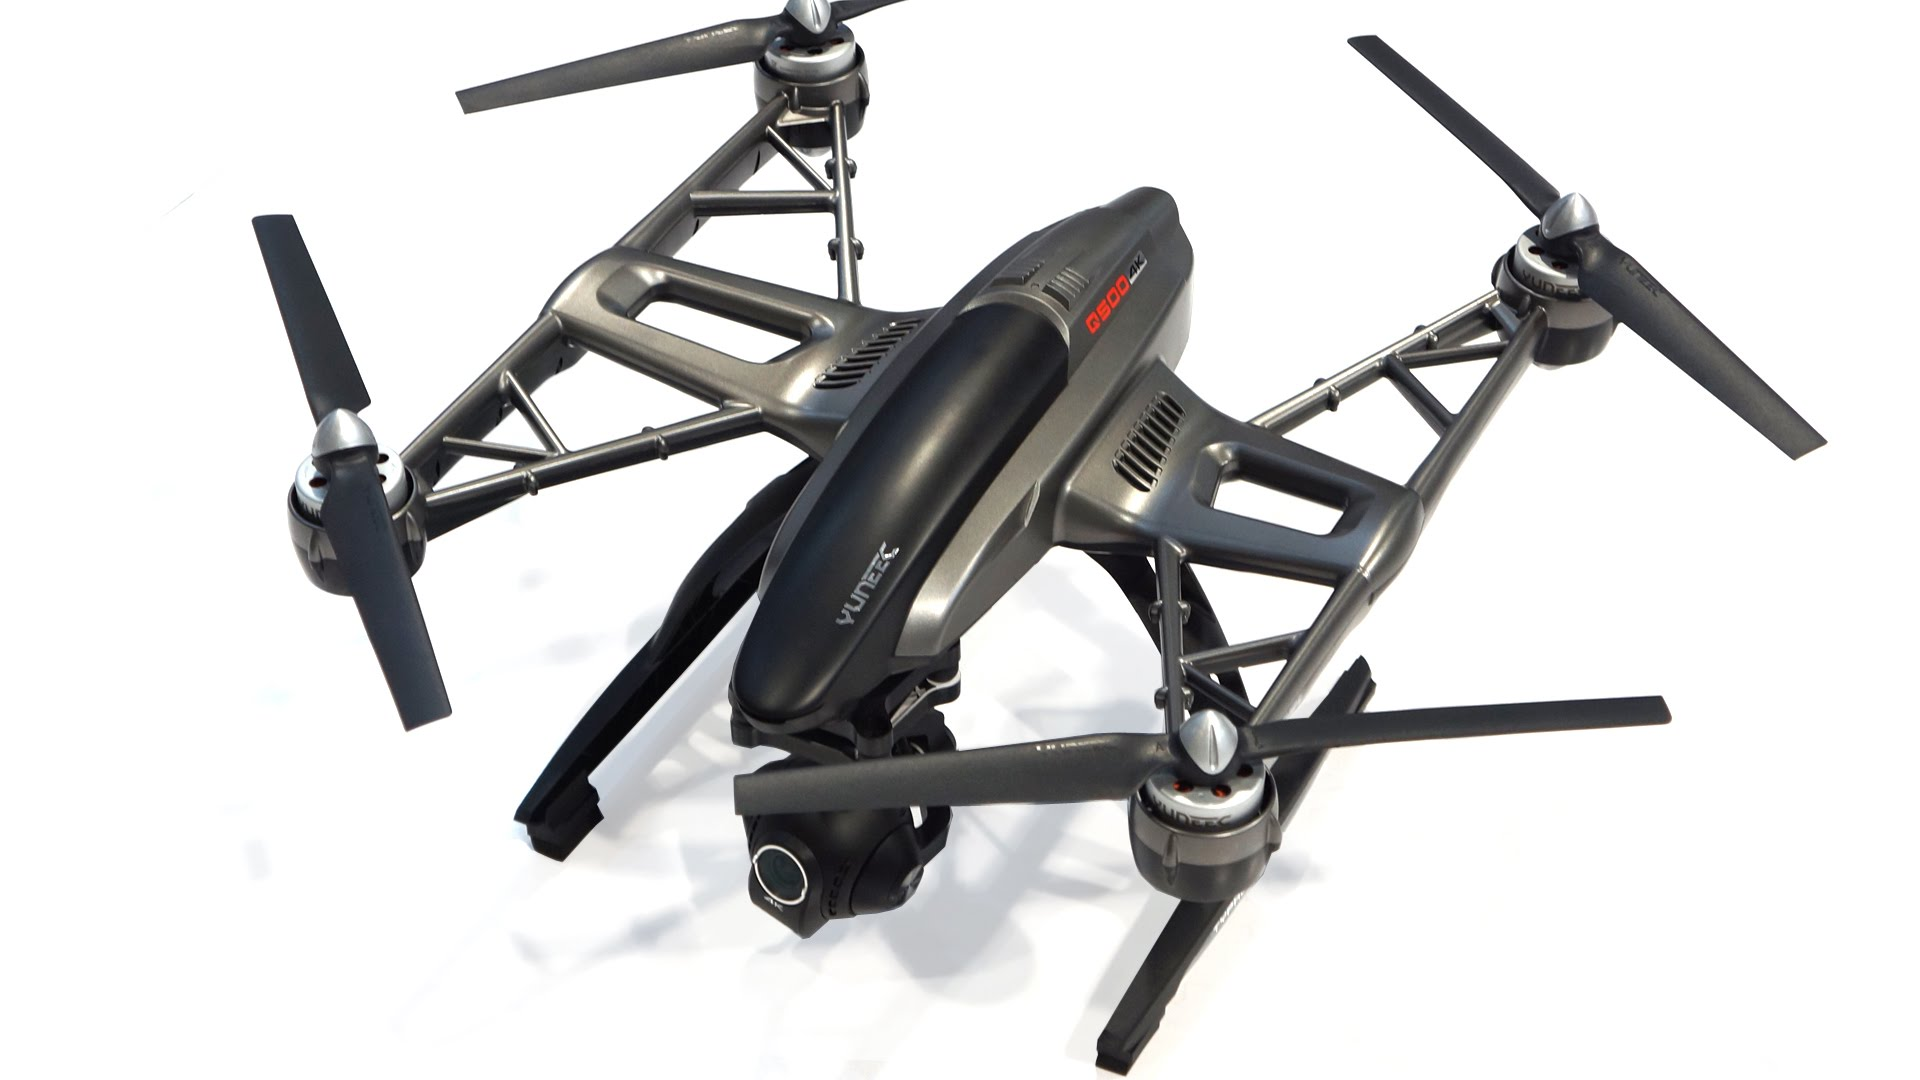
\includegraphics[width=8cm]{drone}
\caption{O drone utilizado para a gravação dos vídeos de teste.}
\label{fig:drone}
\centering
\end{figure}

Para a aquisição das imagens utilizadas para o treinamento da rede, o primeiro vídeo passou por um processo semelhante ao processo de calibração do programa final descrito no Capítulo \ref{cap:solucao}. Duas áreas de interesse foram determinadas de forma idêntica ao processo de escolha de ROIs do \textit{DVE}. Em seguida cada ROI foi dividida em trinta seções verticais. Três quadros do vídeo foram escolhidos de forma aleatória. As imagens correspondentes a cada seção de cada quadro escolhido foram extraídas em arquivos separados. Dessa maneira, as imagens utilizadas para o treinamento da rede neural foram construídas da mesma maneira que as imagens que seriam alimentadas a ela para classificação no futuro.

\section{Treinamento da rede neural artificial}

Uma vez adquiridas as imagens a serem utilizadas para o treinamento, cada uma delas foi separada manualmente em uma das duas categorias:veículo ou vaga vazia. Ao todo foram utilizadas $57$ imagens classificadas como veículo(categoria 1) e $59$ imagens classificadas como vaga vazia(categoria 2) totalizando $116$ imagens. Foram extraídas as características de cada imagem da forma descrita na Seção \ref{sec:extracao}. Os vetores $x_s$ obtidos foram então concatenados de forma a criar duas matrizes. A primeira de dimensões $6\times 57$ representava as \textit{features} das imagens de carros e a segunda de dimensões $6\times 59$ as características das imagens de vagas desocupadas.

\begin{figure}
\centering
\begin{subfigure}{.1\textwidth}
  \centering
  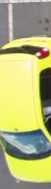
\includegraphics[width=.8\linewidth, height=5cm]{ocupada}
  \caption{}
  \label{fig:exemploRede:sub:ocupada}
\end{subfigure}%
\begin{subfigure}{.1\textwidth}
  \centering
  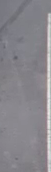
\includegraphics[width=.8\linewidth, height=5cm]{desocupada}
  \caption{}
  \label{fig:exemploRede:sub:desocupada}
\end{subfigure}
\centering
\caption{(a)Um exemplo de imagem classificada manualmente na classe 1.(b) Um exemplo de imagem classificada manualmente na classe 2.}
\label{fig:exemploRede}
\end{figure}

Para que pudesse ser feito o treinamento supervisionado da rede neural, duas matrizes de alvos foram construídas. Uma com dimensões $2\times 57$ e a outra com dimensões $2\times 59$. A primeira matriz com todas as colunas iguais a $\begin{psmallmatrix}1\\0\end{psmallmatrix}$ e a segunda com as colunas da forma $\begin{psmallmatrix}0\\1\end{psmallmatrix}$. Essas matrizes vão compor o gabarito utilizado para o treinamento supervisionado da rede.

As matrizes  de características de cada classe foram então concatenadas formando uma matriz de entrada $In_{6\times 116}$. O mesmo foi feito com as matrizes do gabarito, resultando na matriz $Target_{2\times 116}$. Em seguida as colunas dessas duas matrizes foram reorganizadas aleatoriamente, de forma que as mudanças feitas em $In$ fossem refletidas em $Out$, garantindo que não fosse perdida a relação entre as colunas de mesmo índice das matrizes. O resultado final deste processo é que cada coluna de $Target_{2\times 116}$ indica a classe da coluna correspondente de $In_{6\times 116}$.

Uma vez criadas essas duas matrizes, as entradas e seus respectivos alvos são separados em três conjuntos: o conjunto de treinamento, de validação e de testes. A divisão é feita de forma que $70\%$ das entradas são designadas ao conjunto de treinamento, $15\%$ designadas ao conjunto de validação e os $15\%$ restantes ao conjunto de testes. O conjunto de treinamento então é composto por duas matriz $Ti_{6\times 81}$ e $To_{2\times 81}$ que são iguais as primeira $81$ colunas de $In_{6\times 116}$ e $Target_{2\times 116}$ e representam os vetores descritores das entradas e seus gabaritos respectivamente. Os outros dois conjuntos são construídos de forma similar utilizando. O conjunto de validação é composto por matrizes de $18$ colunas e o de teste por matrizes de $17$ colunas.


A rede neural utilizada foi uma rede \textit{feed-forward} com três camadas. A camada oculta possui $15$ neurônios com função de ativação logística (Equação\ref{eq:logistica}) e a camada de saída $2$ neurônios com função de ativação \textit{softmax} (Equação \ref{eq:softmax}). A rede é submetida a um treinamento supervisionado com um limite de $1000$ iterações. Quando a situação de convergência é atingida, o treinamento para e o resultado é a rede final utilizada.


\section{Resultados Obtidos}

Para determinar a capacidade do \textit{DVE} de determinar se as seções verticais estão ocupadas ou livres, os resultados obtidos pelo programa foram comparados com os resultados que eram esperados de observadores humanos. Foram apresentados a três observadores, que chamaremos pelas iniciais F, M e P, um conjunto de oito vídeos que mostravam veículos estacionando ou saindo de vagas em um estacionamento descoberto. As áreas de interesse do vídeo foram definidas previamente e divididas em $30$ seções verticais. Dessa forma, todos os observadores e o \textit{DVE} analisaram seções verticais idênticas. 

Cada um dos observadores receberam as seguintes instruções:

\begin{itemize}
  \item As regiões de interesse e as seções são numeradas como indicado na Figura \ref{fig:instrucao}.
	\item Uma seção ocupada é aquela cuja maior parte de sua área está ocupada por um veículo.
	\item No momento inicial do vídeo ($0$ segundos), indique quais seções verticais estão ocupadas através do número das ROI e das seções, as outras serão assumidas como livres. Indique também o número de vagas ocupadas.
	\item Se a qualquer momento o estado de ocupação de uma seção mudar, indique o tempo da mudança, a seção onde ocorreu a mudança e a natureza da mudança(ocupada ou liberada).
\end{itemize}

\begin{figure}
\centering
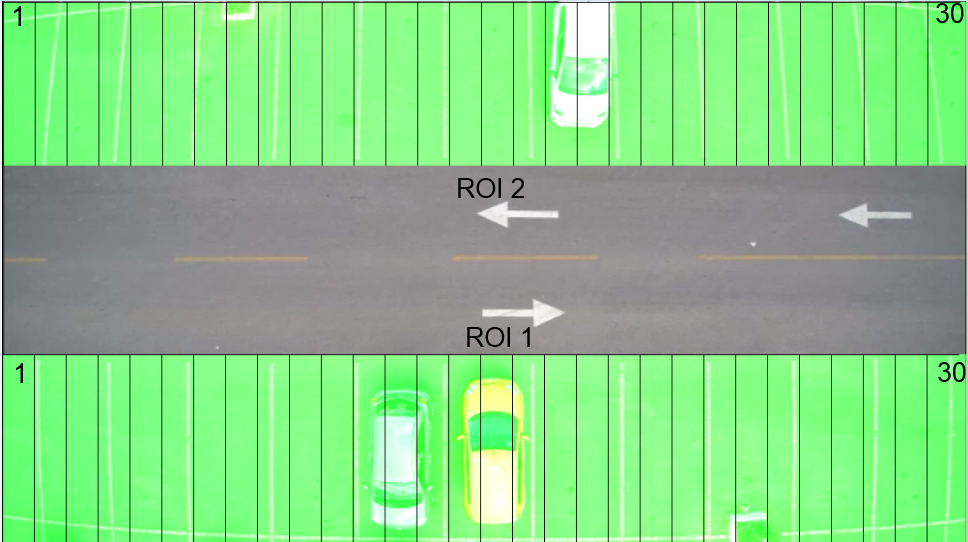
\includegraphics[width=8cm]{instrucoes}
\centering
\caption{Figura mostrando a divisão das ROIs e numeração das seções nos vídeos mostrados para os observadores humanos.}
\label{fig:instrucao}
\end{figure}

Cada observador assistiu aos vídeos sozinho, sem interferência externa e sem conhecimento dos resultados do programa. De fato, a fim de evitar interferência, o \textit{DVE} só foi executado sobre os casos de teste após todos os observadores escolhidos terem entregado os resultados que obteram.

Para os testes apresentados a seguir, serão observadas somente aquelas seções que o \textit{DVE} ou os observadores determinaram como ocupadas. As demais seções serão consideradas livres. Chamaremos de um \textit{acerto} sempre que em um determinado segundo $t$, o programa e um observador concordam quanto a ocupação de uma seção vertical. Sendo assim, o programa pode atingir um máximo de $60$ acertos por segundo. A indicação da ocupação das seções pelos observadores não foi definida a cada segundo, mas considera-se que entre duas acusações de mudança de estado a ocupação das seções permanece a mesma. Sendo assim, podemos utilizar esses momentos para definir a ocupação em cada segundo do vídeo. Por exemplo, se um observador disser que a seção $10$ estava ocupada no momento inicial do vídeo e depois indicar que a mesma sessão foi liberada aos $8s$, a seção será considerada ocupada durante todos os momentos deste intervalo. 

Além da capacidade de classificar cada seção, a precisão do \textit{DVE} em determinar o número de vagas ocupadas a cada momento do vídeo também foi analisada. Para este teste, os observadores foram instruídos a informar o número de vagas ocupadas no início do vídeo. Sempre que considerassem que houve uma mudança neste número, deveriam informar o momento da mudança e o novo número de vagas ocupadas. Para esta análise, um \textit{acerto} é considerado a cada segundo que o programa indica o mesmo número de vagas ocupadas que os observadores. Para a determinação das vagas o programa foi executado no modo complexo de mapeamento.

Nas seções seguintes serão apresentados cada um dos vídeos utilizados para os testes. Cada caso iniciará com uma breve descrição do movimento dos veículos no vídeo, a duração do vídeo e o número de acertos possíveis para as seções verticais, seguidos de cinco tabelas, uma para cada observador e duas para o \textit{DVE}. As tabelas indicam o tempo onde foram acusadas mudanças de estado nas seções e no número de vagas ocupadas. A primeira linha da tabela indica as seções ocupadas no momento inicial do vídeo e cada linha subsequente indica um momento em segundos quando houve mudança de estado de pelo menos uma seção ou vaga, a ROI e o número das seções modificadas e o número de vagas ocupadas naquele momento no tempo.  Finalmente, será calculada uma taxa de acerto que compara o desempenho do programa na classificação a cada observador e uma taxa final de acerto média para o caso de teste. A taxa de acerto para cada observador é calculada pela razão entre o número de acertos do programa e o número de acertos possíveis para o caso de teste e a taxa de acerto média é a média aritmética entre estes valores. Para que o leitor possa comparar o desempenho do \textit{DVE} com suas próprias impressões, uma imagem dos momentos iniciais e finais de cada vídeo será mostrada junto de cada análise.

A leitura das tabelas que representam as taxas de acerto devem ser feitas com um certo cuidado. Por causa da grande quantidade de seções e de possíveis acertos, um erro na classificação de uma seção representa uma mudança pequena na taxa de acerto. Em cada caso de testes há um grande número de seções aonde não há movimento algum, que são classificadas corretamente como vazias, elevando a taxa de acertos do teste. Enquanto esses acertos são relevantes, a classificação correta das seções onde há movimento de veículos representa uma diferença muito maior no funcionamento do \textit{DVE}.

Por outro lado, a taxas de acerto das ocupações das vagas são muito mais afetadas por erros. Se o \textit{DVE} indicar uma vaga ocupada a mais que um observador por apenas $1$ segundo, um erro quase insignificante em termos humanos, isso pode representar uma diminuição de até $10\%$ na taxa de acerto. 

Por isso, as taxas de acerto não são fatores exclusivos na determinação da eficácia do programa. Assim, uma análise rápida do comportamento do \textit{DVE} em cada caso de testes será apresentada após as tabelas.

\subsection{Vídeo 1}

No primeiro caso de testes, o vídeo começa com um estacionamento vazio. Depois de alguns segundos um único veículo de cor branca entra na cena pela direita e estaciona em uma vaga na parte inferior da imagem. O vídeo tem $15s$ de duração, totalizando $900$ acertos possíveis.

\begin{figure}[!h]
\centering
\begin{subfigure}{.5\textwidth}
\centering
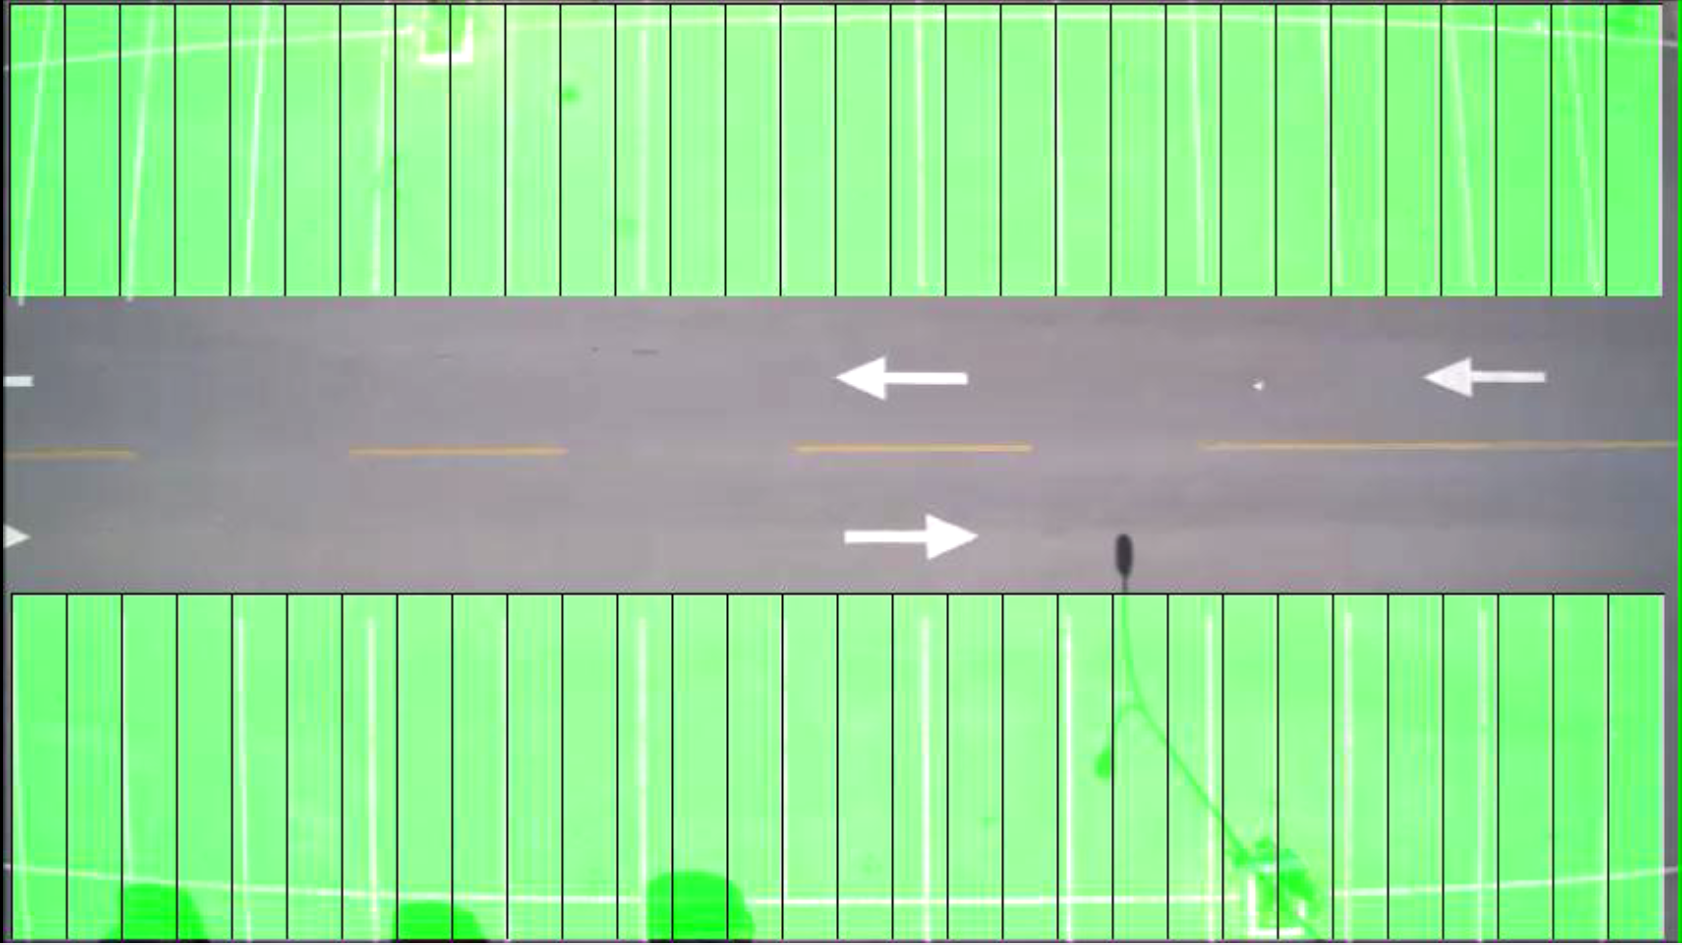
\includegraphics[width=.8\linewidth]{Video1Inicio}
\caption{}
\end{subfigure}\
\begin{subfigure}{.5\textwidth}
\centering
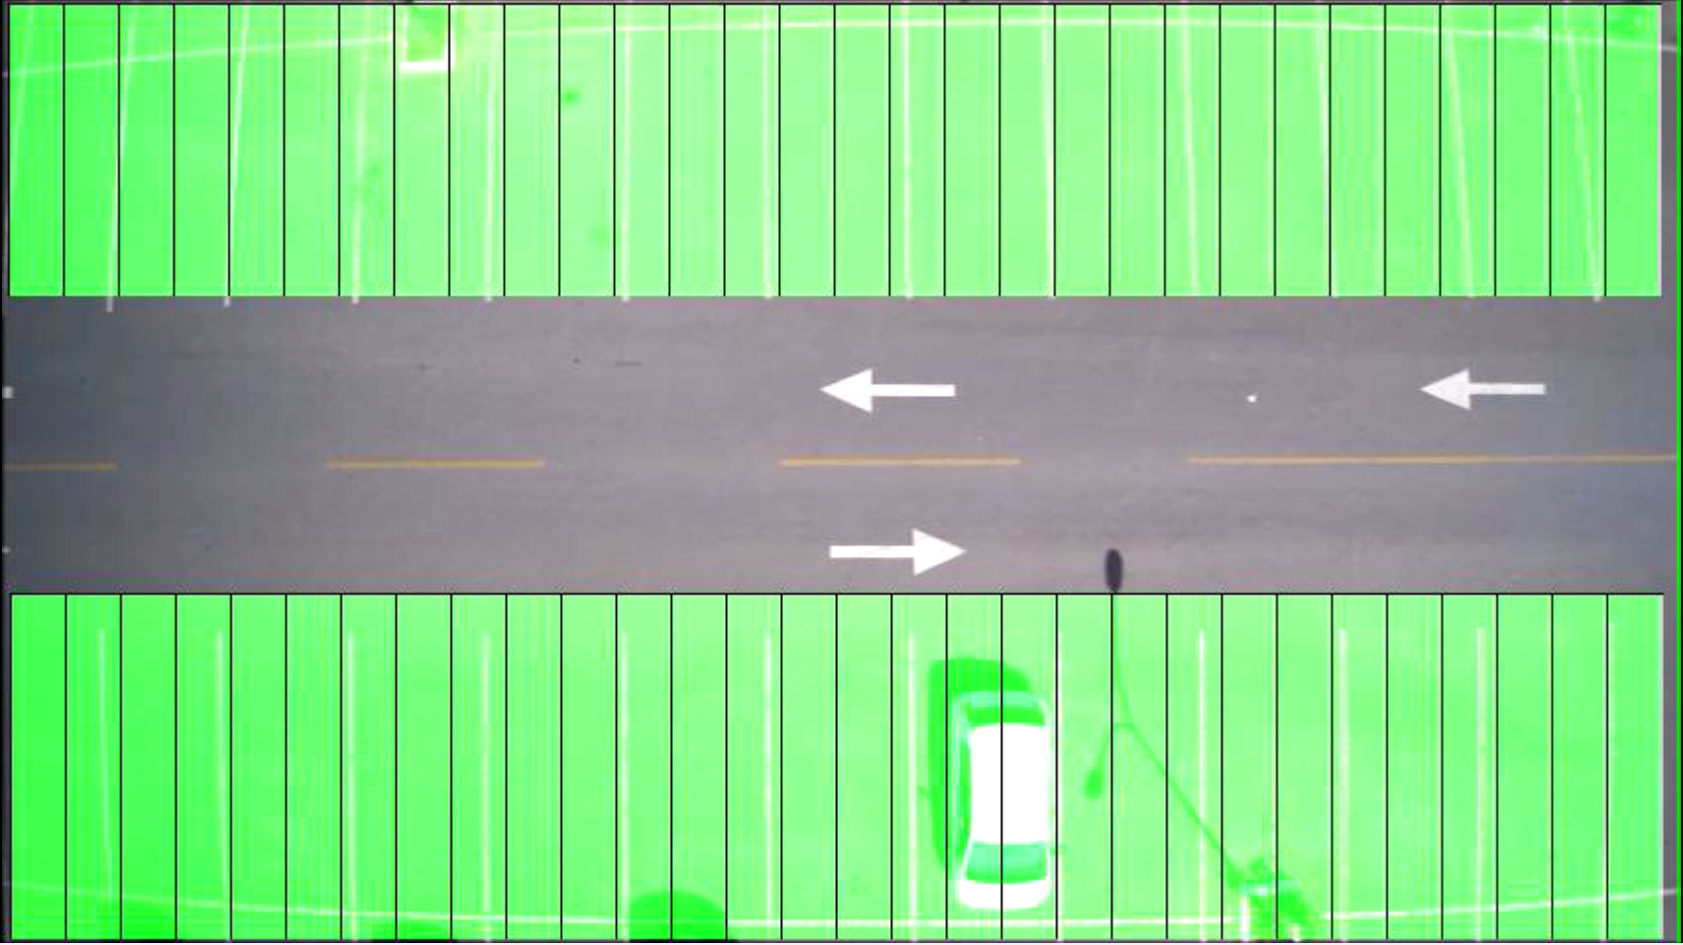
\includegraphics[width=.8\linewidth]{Video1Fim}
\caption{}
\end{subfigure}
\centering
\caption{(a) O momento inicial do vídeo 1; (b) O momento final do vídeo 1.}%
\label{}%
\end{figure}


\begin{center}
\begin{tabular}{|c||c||c|}
\hline
\multicolumn{3}{|c|}{Observador F}  \\ \hline \hline
Tempo(s) & Acontecimento & Vagas ocupadas\\ \hline
0 & Nenhuma seção ocupada & 0 \\ \hline
10 & ROI 2: Seções 18 e 19 ocupadas. & 1 \\
\hline
\end{tabular}
\end{center}

\begin{center}
\begin{tabular}{|c||c||c|}
\hline
\multicolumn{3}{|c|}{Observador P}  \\ \hline \hline
Tempo(s) & Acontecimento & Vagas ocupadas\\ \hline
0 & Nenhuma seção ocupada & 0 \\ \hline
10 & ROI 2: Seções 18 e 19 ocupadas. & 1 \\
\hline
\end{tabular}
\end{center}

\begin{center}
\begin{tabular}{|c||c||c|}
\hline
\multicolumn{3}{|c|}{Observador M}  \\ \hline \hline
Tempo(s) & Acontecimento & Vagas ocupadas\\ \hline
0 & Nenhuma seção ocupada & 0 \\ \hline
9 & ROI 2: Seções 18 e 19 ocupadas. & 1 \\
\hline
\end{tabular}
\end{center}

\begin{center}
\begin{tabular}{|c||c||c|}
\hline
\multicolumn{3}{|c|}{DVE}  \\ \hline \hline
Tempo(s) & Acontecimento & Vagas Ocupadas\\ \hline
0 & ROI 2:Seção 3 ocupada. & 1 \\ \hline
10 & ROI 2: Seções 18 e 19 ocupadas. & 2\\ \hline
14 & ROI 2: Seção 3 liberada. & 1\\
\hline
\end{tabular}
\end{center}

\begin{center}
\begin{tabular}{|c||c||c|}
\hline
\multicolumn{3}{|c|}{Acertos - seções}  \\ \hline \hline
Observador & Acertos& Taxa de acertos \\ \hline
F & 886 & 98,44\% \\  \hline
P & 886 & 98,44\% \\ \hline
M & 884 & 98,22\% \\ \hline
Média & 885,3 & 98,37\% \\
\hline
\end{tabular}
\end{center}

\begin{center}
\begin{tabular}{|c||c||c|}
\hline
\multicolumn{3}{|c|}{Acertos - vagas}  \\ \hline \hline
Observador & Acertos & Taxa de acertos \\ \hline
F & 1 & 7\% \\  \hline
P & 1 & 7\% \\ \hline
M & 1 & 7\% \\ \hline
Média & 1 & 7\% \\
\hline
\end{tabular}
\end{center}

Neste caso de testes, o programa classifica errôneamente a seção $3$ da ROI $2$ durante quase toda a duração do vídeo. Como o erro se inicia logo no primeiro momento do vídeo, esta seção é definida como uma vaga que conta como ocupada enquanto o erro de classificação persiste, fazendo com que o programa indique um número de vagas ocupadas errado durante toda a sua execução. Esse caso ilustra uma possível consequência de um erro de classificação. Apesar do erro, o reconhecimento da vaga ocupada pelo veículo nas seções $18$ e $19$ ocorre sem problemas.

\subsection{Vídeo 2}

Neste vídeo, um carro branco está estacionado no conjunto inferior de vagas. Um veículo cinza entra pela direita e estaciona no conjunto superior de vagas. O vídeo tem uma duração de $10s$, totalizando $600$ acertos possíveis.

\begin{figure}[!h]
\centering
\begin{subfigure}{.5\textwidth}
\centering
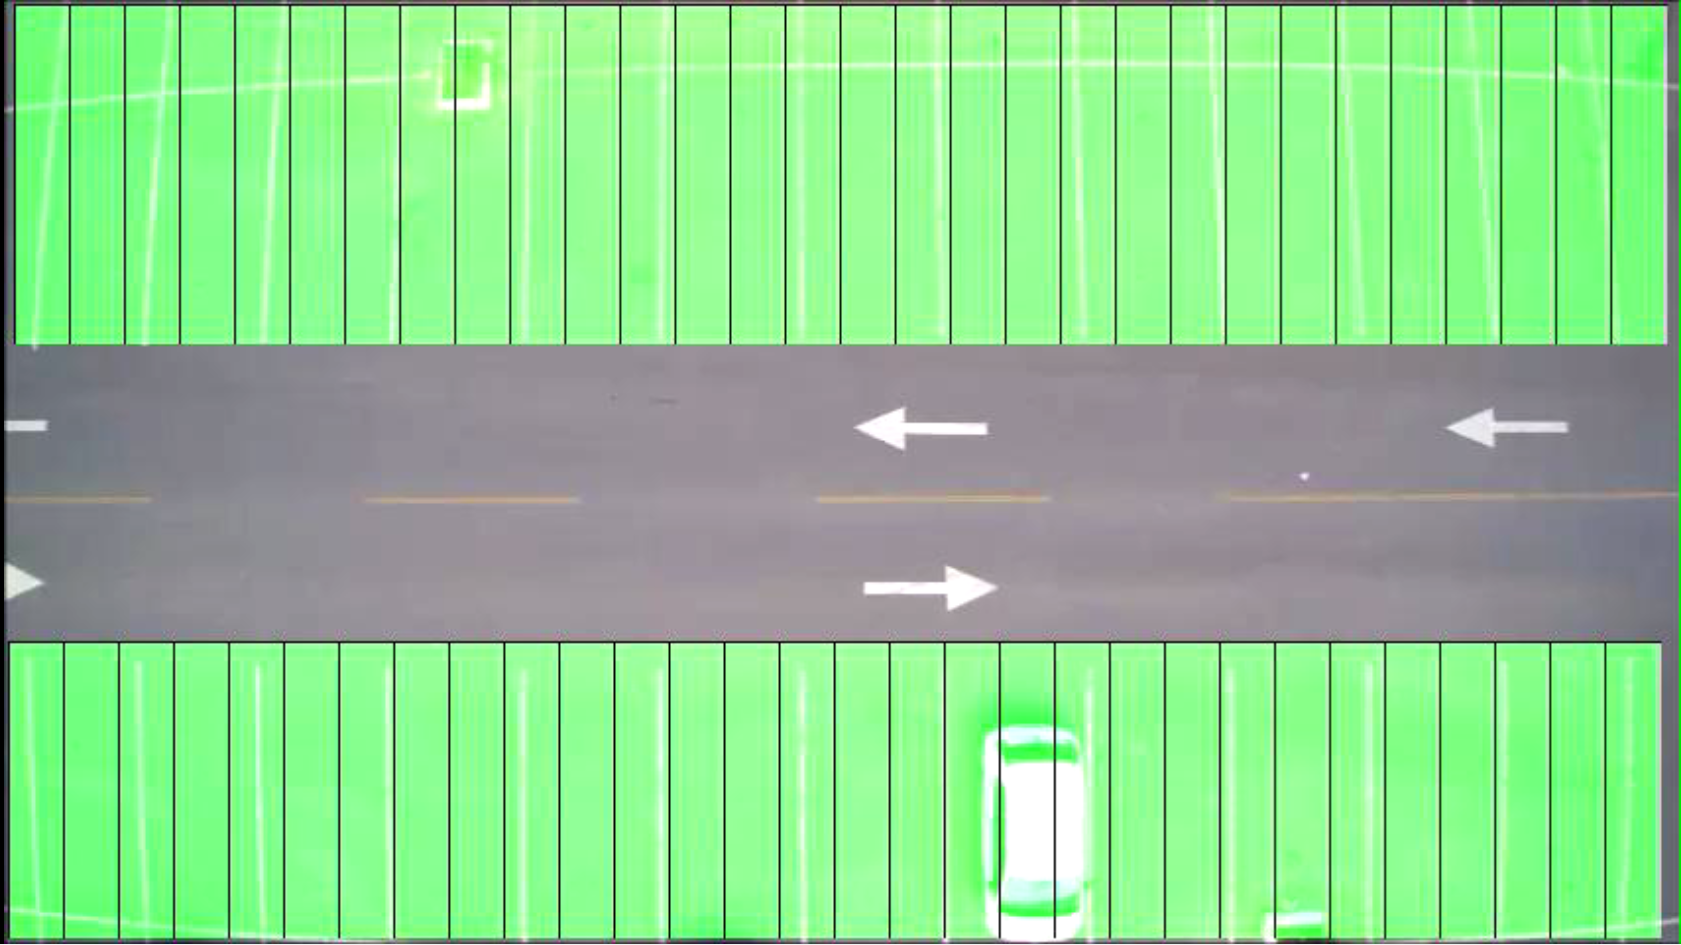
\includegraphics[width=.8\linewidth]{Video2Inicio}
\caption{}
\end{subfigure}\
\begin{subfigure}{.5\textwidth}
\centering
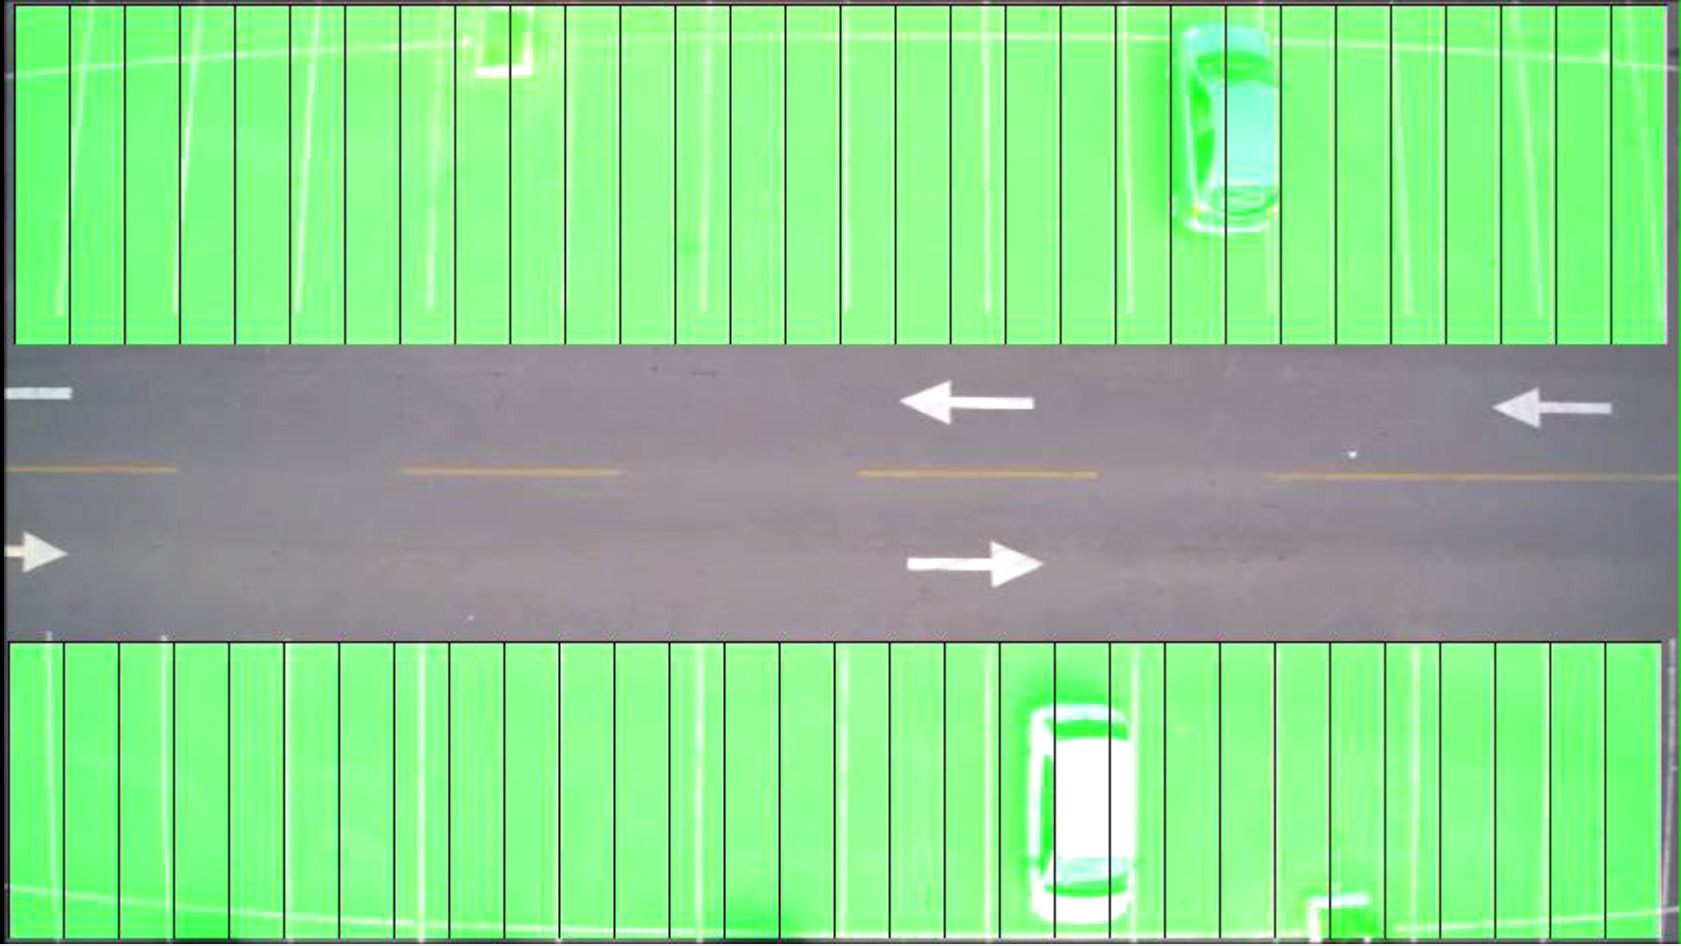
\includegraphics[width=.8\linewidth]{Video2Fim}
\caption{}
\end{subfigure}
\centering
\caption{(a) O momento inicial do vídeo 2; (b) O momento final do vídeo 2.}%
\label{}%
\end{figure}


\begin{center}
\begin{tabular}{|c||c||c|}
\hline
\multicolumn{3}{|c|}{Observador F}  \\ \hline \hline
Tempo(s) & Acontecimento & Vagas Ocupadas\\ \hline
0 & ROI 2: Seções 19 e 20 ocupadas & 1 \\ \hline
6 & ROI 1: Seções 21,22 e 23 ocupadas. & 2 \\
\hline
\end{tabular}
\end{center}

\begin{center}
\begin{tabular}{|c||c||c|}
\hline
\multicolumn{3}{|c|}{Observador P}  \\ \hline \hline
Tempo(s) & Acontecimento & Vagas Ocupadas\\ \hline
0 & ROI 2: Seções 19 e 20 ocupadas  & 1\\ \hline
6 & ROI 1: Seções 20,21,22 ocupadas. & 2 \\
\hline
\end{tabular}
\end{center}

\begin{center}
\begin{tabular}{|c||c||c|}
\hline
\multicolumn{3}{|c|}{Observador M}  \\ \hline \hline
Tempo(s) & Acontecimento & Vagas Ocupadas\\ \hline
0 & ROI 2: Seções 19 e 20 ocupadas & 1\\ \hline
6 & ROI 1: Seções 21,22 e 23 ocupadas. & 2\\
\hline
\end{tabular}
\end{center}

\begin{center}
\begin{tabular}{|c||c||c|}
\hline
\multicolumn{3}{|c|}{DVE}  \\ \hline \hline
Tempo(s) & Acontecimento & Vagas Ocupadas\\ \hline
0 & ROI 2: Seções 18,19 e 20 ocupadas. & 1 \\ \hline
6 & ROI 1: Seções 21 e 22 ocupadas. & 2 \\ \hline
\hline
\end{tabular}
\end{center}

\begin{center}
\begin{tabular}{|c||c||c|}
\hline
\multicolumn{3}{|c|}{Acertos - seções}  \\ \hline \hline
Observador & Acertos & Taxa de acertos \\ \hline
F & 586 & 97,66\% \\  \hline
P & 586 & 97,66\% \\ \hline
M & 586 & 97,66\% \\ \hline
Média & 586 & 97,66\% \\
\hline
\end{tabular}
\end{center}

\begin{center}
\begin{tabular}{|c||c||c|}
\hline
\multicolumn{3}{|c|}{Acertos - vagas}  \\ \hline \hline
Observador & Acertos & Taxa de acertos \\ \hline
F & 10 & 100\% \\  \hline
P & 10 & 100\% \\ \hline
M & 10 & 100\% \\ \hline
Média & 10 & 100\% \\
\hline
\end{tabular}
\end{center}

Neste caso de testes, houve discordância entre os observadores sobre as seções ocupadas pelo carro cinza na parte superior do vídeo. Porém o \textit{DVE} classificou como ocupadas as seções onde houve consenso entre os observadores.

O programa também classificou errôneamente a seção $18$ do ROI $2$ no momento inicial do vídeo. Novamente ele acerta nas seções onde há consenso entre os observadores. O erro é mais aceitável que o erro que ocorreu no vídeo $1$, pois a determinação da vaga ainda ocorre de maneira que a sua ocupação é reconhecida.

\subsection{Vídeo 3}

Neste vídeo, dois carros se encontram no estacionamento. Um veículo amarelo entra pela direita e estaciona na seção superior das vagas. O veículo branco sai pela parte de baixo da tela. Ele tem duração de $20s$ totalizando $1200$ acertos possíveis.

\begin{figure}[!h]
\centering
\begin{subfigure}{.5\textwidth}
\centering
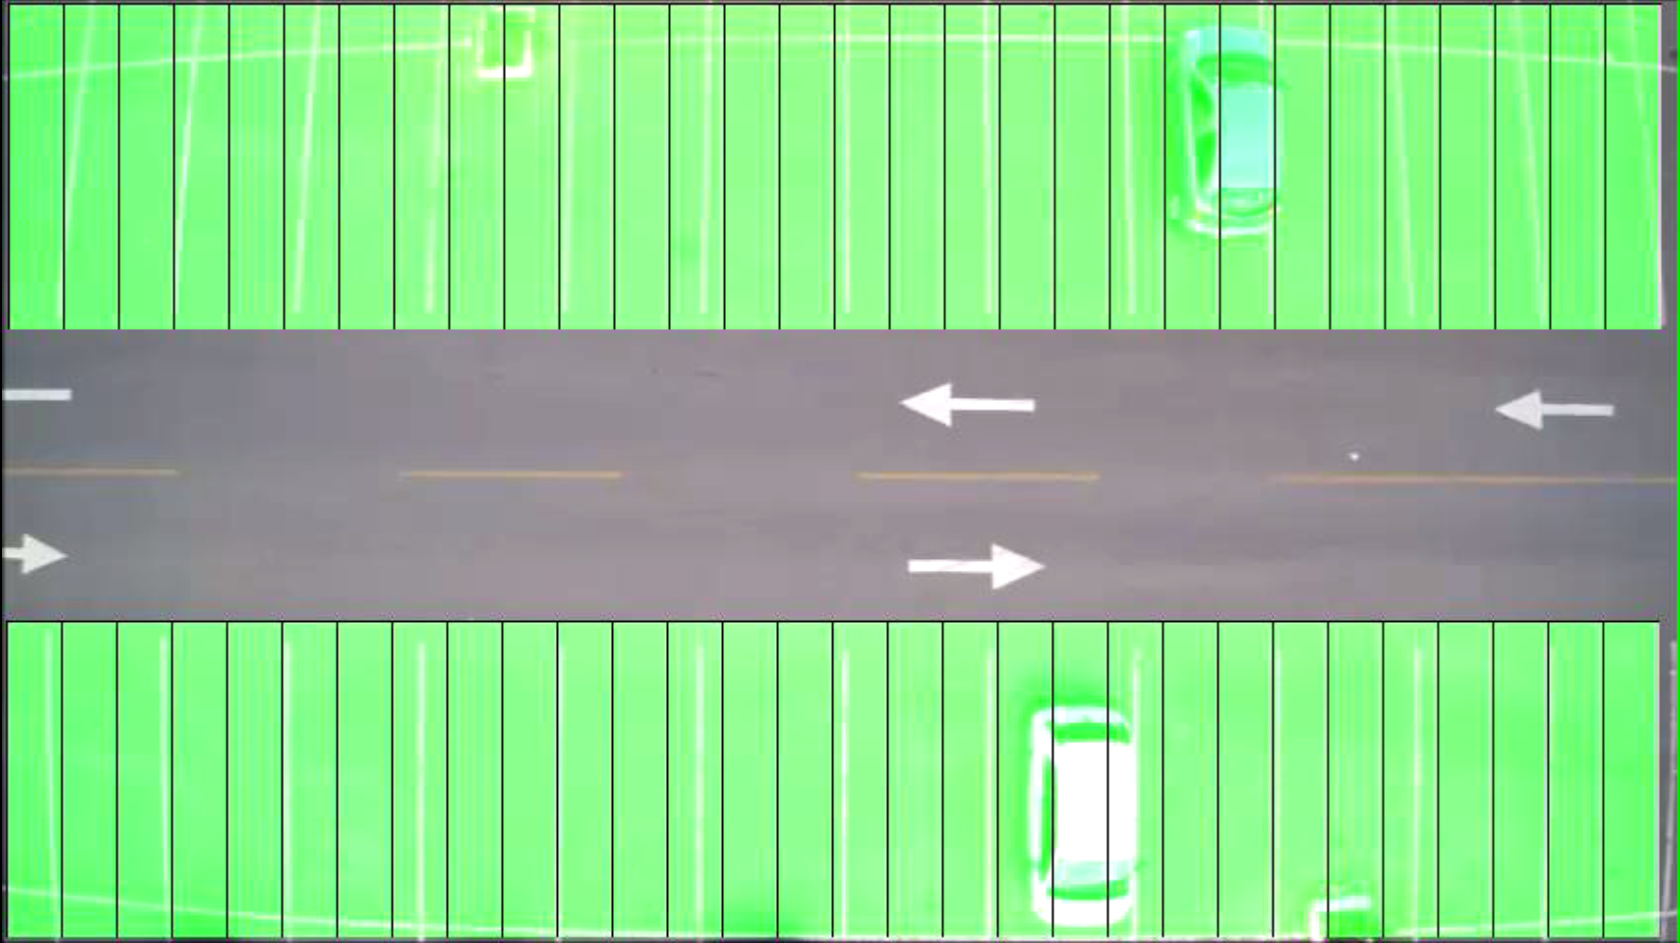
\includegraphics[width=.8\linewidth]{Video3Inicio}
\caption{}
\end{subfigure}\
\begin{subfigure}{.5\textwidth}
\centering
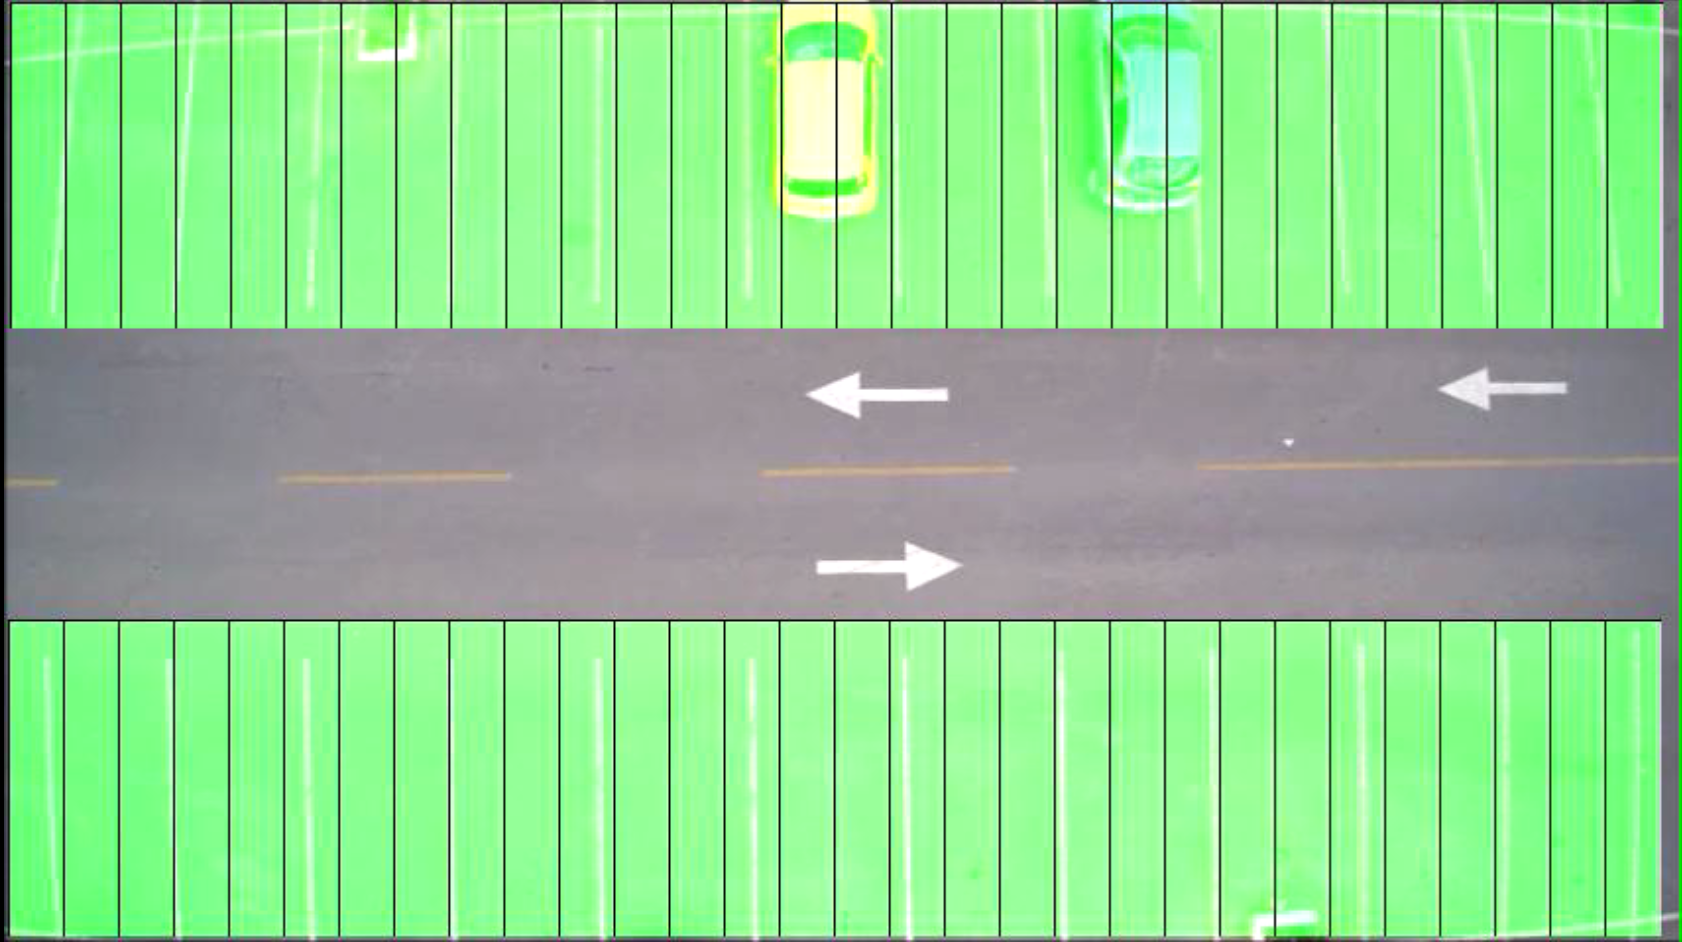
\includegraphics[width=.8\linewidth]{Video3Fim}
\caption{}
\end{subfigure}
\centering
\caption{(a) O momento inicial do vídeo 3; (b) O momento final do vídeo 3.}%
\label{}%
\end{figure}

\begin{center}
\begin{tabular}{|c||c||c|}
\hline
\multicolumn{3}{|c|}{Observador F}  \\ \hline \hline
Tempo(s) & Acontecimento & Vagas Ocupadas\\ \hline
0 & ROI 1: Seções 22 e 23 ocupadas. & 2 \\
 & ROI 2: 19,20 e 21 ocupadas & \\ \hline
8 & ROI 1: Seções 16 e 17 ocupadas. & 3\\ \hline
13 & ROI 2: Seções 18 e 19 liberadas. & 2\\
\hline
\end{tabular}
\end{center}

\begin{center}
\begin{tabular}{|c||c||c|}
\hline
\multicolumn{3}{|c|}{Observador P}  \\ \hline \hline
Tempo(s) & Acontecimento & Vagas Ocupadas\\ \hline
0 & ROI 1: Seções 22 e 23 ocupadas. & 2 \\
 & ROI 2: 20 e 21 ocupadas &  \\ \hline
9 & ROI 1: Seções 15,16 e 17 ocupadas. & 3 \\
\hline
\end{tabular}
\end{center}

\begin{center}
\begin{tabular}{|c||c||c|}
\hline
\multicolumn{3}{|c|}{Observador M}  \\ \hline \hline
Tempo(s) & Acontecimento & Vagas Ocupadas\\ \hline
0 & ROI 1: Seções 22 e 23 ocupadas. & 2 \\
 & ROI 2: 20 e 21 ocupadas & \\ \hline
8 & ROI 1: Seções 15,16 e 17 ocupadas. & 3 \\ \hline
14 & ROI 2: Seções 17,18 e 19 liberadas & 2\\
\hline
\end{tabular}
\end{center}

\begin{center}
\begin{tabular}{|c||c||c|}
\hline
\multicolumn{3}{|c|}{DVE}  \\ \hline \hline
Tempo(s) & Acontecimento & Vagas Ocupadas\\ \hline
0 & ROI 1: Seções 22 e 23 ocupadas. & 2 \\
 & ROI 2: 19,20 e 21 ocupadas &  \\ \hline
1 & ROI 1: Seção 23 liberada. & 2 \\ \hline
2 & ROI 1: Seção 23 ocupada. & 2 \\ \hline
4 & ROI 1: Seção 23 liberada. & 2 \\ \hline
8 & ROI 1: Seções 16 e 17 ocupadas. & 3 \\ \hline
9 & ROI 2: Seção 21 liberada. & 3 \\ 
 & ROI 2: Seções 18 e 24 ocupadas &  \\ \hline
10 & Sem acontecimentos & 2 \\ \hline
11 & ROI 1: Seção 20 ocupada. & 3 \\ 
 & ROI 2: Seção 24 liberada. \\ \hline
13 & ROI 1: Seção 20 liberada. & 2 \\
 & ROI 2: Seção 18,19 e 20 liberada. & \\ \hline
16 & ROI 1: Seção 20 ocupada. & 2 \\ \hline
19 & ROI 1: Seção 20 liberada. & 2 \\
\hline
\end{tabular}
\end{center}

\begin{center}
\begin{tabular}{|c||c||c|}
\hline
Observador & Acertos & Taxa de acertos \\ \hline
F & 1165 & 97,08\% \\  \hline
P & 1113 & 92,75\% \\ \hline
M & 1136 & 94,66\% \\ \hline
Média & 1138 & 94,83\% \\
\hline
\end{tabular}
\end{center}

\begin{center}
\begin{tabular}{|c||c||c|}
\hline
\multicolumn{3}{|c|}{Acertos - vagas}  \\ \hline \hline
Observador & Acertos & Taxa de acertos \\ \hline
F & 19 & 95\% \\  \hline
P & 11 & 55\% \\ \hline
M & 18 & 90\% \\ \hline
Média & 16 & 80\% \\
\hline
\end{tabular}
\end{center}



Esse caso de teste possui alguns problemas causados principalmente por causa da movimentação do \textit{drone} no momento da gravação. Essa movimentação faz com que partes da imagem passem a ocupar seções diferentes, criando algumas incosistências. Repare que por volta dos $14s$ dois dos observadores disseram que a seção $18$ da ROI $2$ foi liberada, apesar de nunca terem acusado que ela estava ocupada anteriormente. Essa inconsistência ocorre porque entre o início do vídeo esse momento, o \textit{drone} utilizado para a gravação se movimenta e faz com que o veículo que estava ocupando as  seções $19$ e $20$ ocupe as seções $18$ e $19$. Esse problema acontece em outros casos de teste em menor proporção.

O teste sobre esse vídeo ainda possui resultados interessantes e úteis. Uma vantagem do uso de um sistema automatizado se mostra neste caso de teste. O observador \textit{P} não percebeu que um veículo saia da tela por volta dos $14$ segundos e por isso não acusou a mudança de estado de nenhuma seção nesse momento. Uma falha que não ocorre no programa.

Através deste caso também percebe-se que o \textit{DVE} tem dificuldade em classificar corretamente as seções ocupadas pelo veículo cinza na ROI $1$, evidenciada principalmente pela flutuação da classificação das seções $23$ e $20$.

Mesmo com os problemas, o mapeamento e determinação das ocupações das vagas mostra uma alta taxa de acerto. Neste caso de teste, a determinação inicial das vagas funciona a favor do programa. Apesar de ter dificuldades em classificar o carro cinza, o \textit{DVE} identifica uma das seções que ele ocupa e determina que esta seção pertence a uma vaga. Por isso, o número de vagas ocupadas se mantém correto durante a execução do teste. Uma flutuação na classificação da seção causa um erro por um segundo, mas que é rapidamente corrigido. Além disso o sistema de mapeamento se mostrou eficaz e seguro. Quando o deslocamento do drone ocorre, diversos movimentos são detectados no vídeo, causando a marcação de várias vagas. Apesar disso, nenhuma seção fica marcada em duas vagas.



\subsection{Vídeo 4}

Neste vídeo, o veículo branco entra em cena pela parte superior da tela e estaciona entre os outros dois carros. O carro cinza sai da vaga que ocupava e estaciona em uma na área inferior. O vídeo possui uma duração de $30s$, portanto $1800$ possíveis acertos.

\begin{figure}[!h]
\centering
\begin{subfigure}{.5\textwidth}
\centering
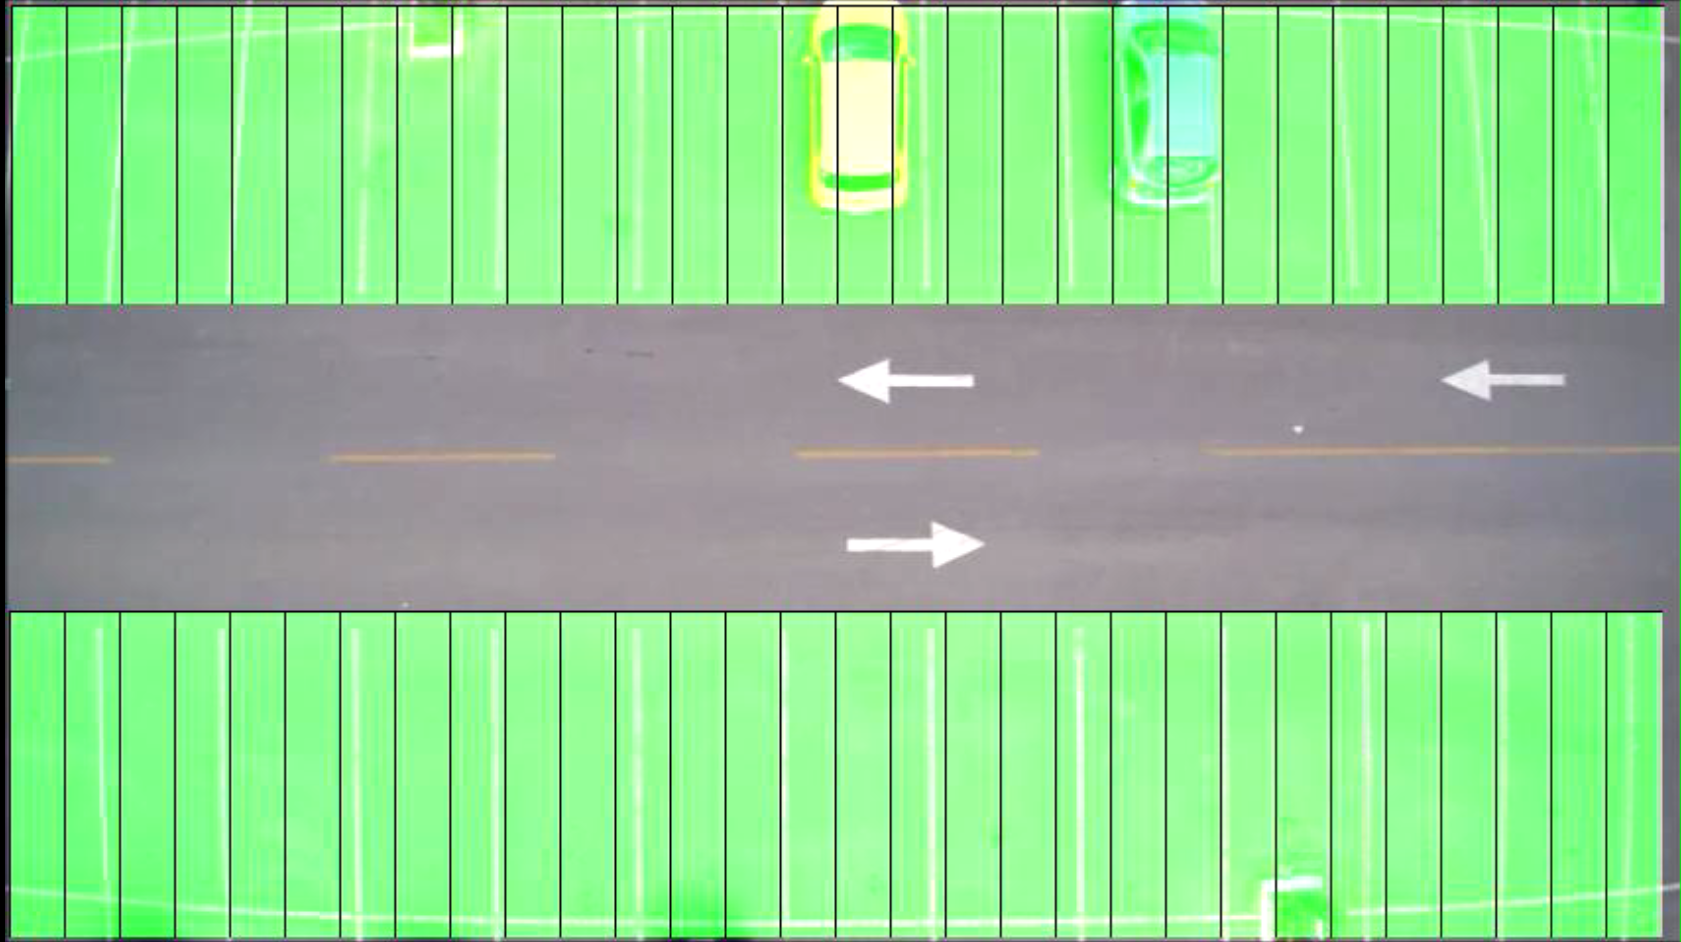
\includegraphics[width=.8\linewidth]{Video4Inicio}
\caption{}
\end{subfigure}\
\begin{subfigure}{.5\textwidth}
\centering
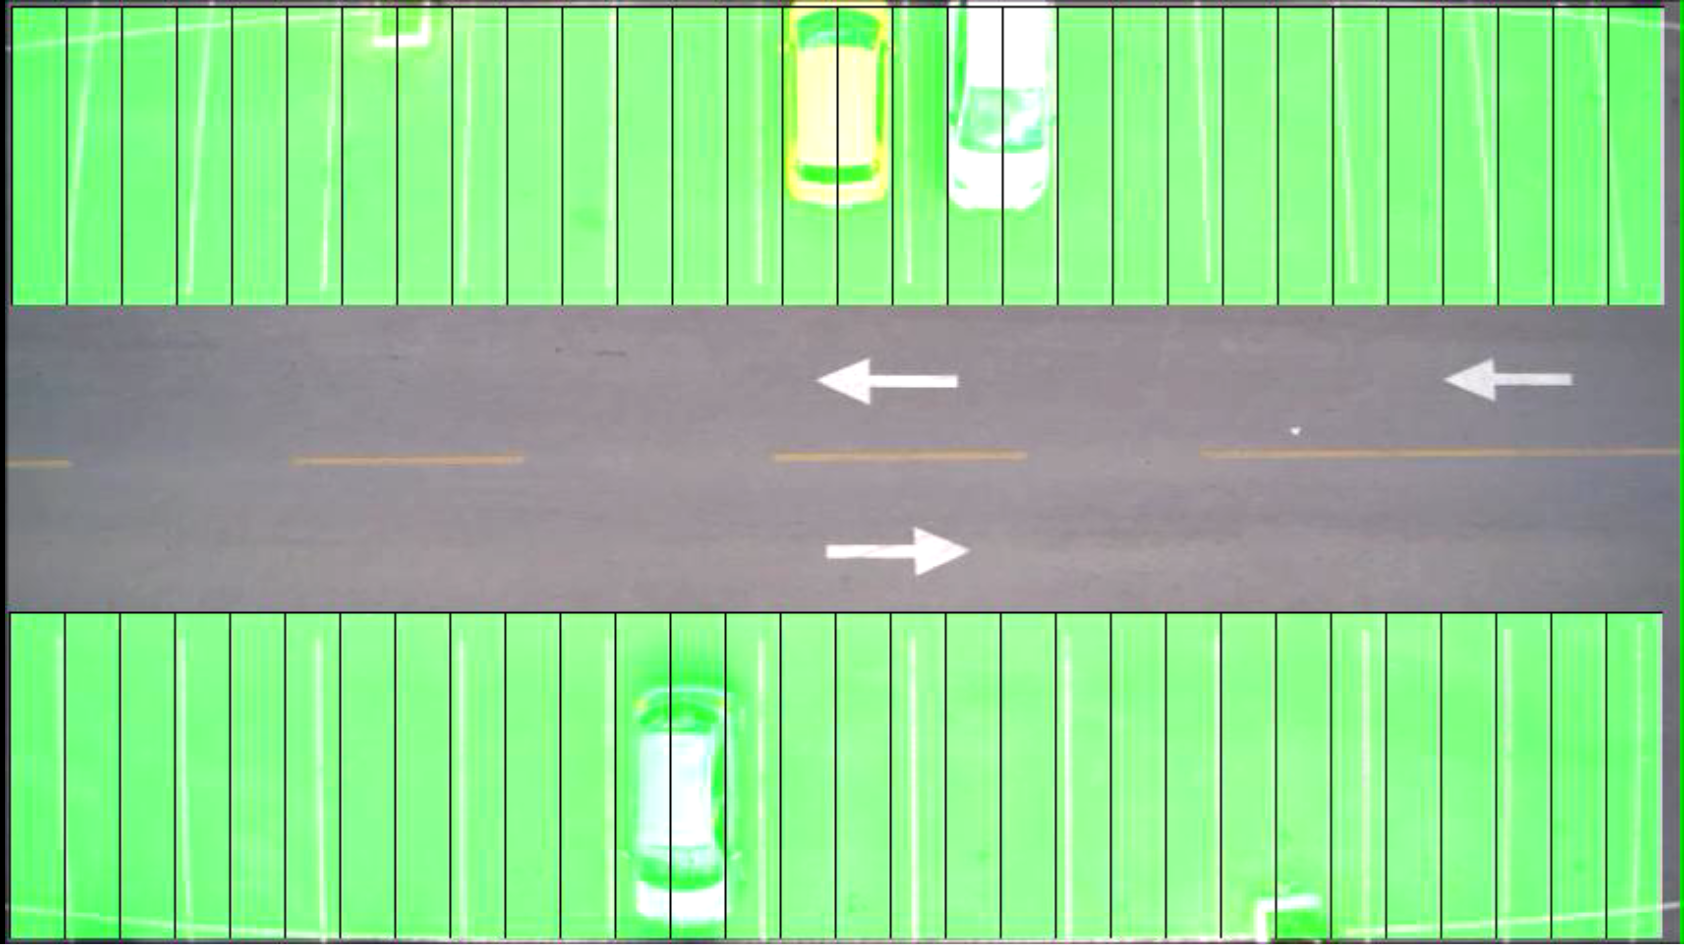
\includegraphics[width=.8\linewidth]{Video4Fim}
\caption{}
\end{subfigure}
\centering
\caption{(a) O momento inicial do vídeo 4; (b) O momento final do vídeo 4.}%
\label{}%
\end{figure}

\begin{center}
\begin{tabular}{|c||c||c|}
\hline
\multicolumn{3}{|c|}{Observador F}  \\ \hline \hline
Tempo(s) & Acontecimento & Vagas Ocupadas\\ \hline
0 & ROI 1: Seções 15,16,21 e 22 ocupadas. & 2 \\ \hline
7 & ROI 1: Seções 19 e 20 ocupadas. & 3 \\ \hline
16 & ROI 1: Seções 21 e 22 liberadas. & 2 \\ \hline
28 & ROI 2: Seções 12 e 13 ocupadas. & 3 \\
\hline
\end{tabular}
\end{center}

\begin{center}
\begin{tabular}{|c||c||c|}
\hline
\multicolumn{3}{|c|}{Observador P}  \\ \hline \hline
Tempo(s) & Acontecimento & Vagas Ocupadas\\ \hline
0 & ROI 1: Seções 15,16,17,20 e 21 ocupadas. & 2 \\ \hline
8 & ROI 1: Seções 18 e 19 ocupadas. & 3 \\ \hline
18 & ROI 1: Seções 21 e 22 liberadas & 2 \\ \hline
29 & ROI 2: 12,13 e 14 ocupadas & 3 \\
\hline
\end{tabular}
\end{center}

\begin{center}
\begin{tabular}{|c||c||c|}
\hline
\multicolumn{3}{|c|}{Observador M}  \\ \hline \hline
Tempo(s) & Acontecimento & Vagas Ocupadas\\ \hline
0 & ROI 1: Seções 15,16,20 e 21 ocupadas. & 2 \\ \hline
6 & ROI 1: Seções 18 e 19 ocupadas. & 3 \\ \hline
17 & ROI 1: Seções 21 e 22 liberadas & 2 \\ \hline
28 & ROI 2: Seções 12,13 e 14 ocupadas & 3 \\
\hline
\end{tabular}
\end{center}

\begin{center}
\begin{tabular}{|c||c||c|}
\hline
\multicolumn{2}{|c|}{DVE}  \\ \hline \hline
Tempo(s) & Acontecimento & Vagas Ocupadas\\ \hline
0 & ROI 1: Seções 15,16,20 e 21 ocupadas. & 2 \\ \hline
6 & ROI 1: Seções 18 e 19 ocupadas. & 3 \\ \hline
11 & ROI 1: Seção 22 ocupada. & 3 \\ \hline
14 & ROI 1: Seção 22 liberada. & 3 \\ \hline
23 & ROI 1: Seção 20 liberada. & 2 \\ \hline
28 & ROI 2: Seções 12 e 13 ocupadas. & 3 \\
\hline
\end{tabular}
\end{center}

\begin{center}
\begin{tabular}{|c||c||c|}
\hline
\multicolumn{3}{|c|}{Acertos - seções}  \\ \hline \hline
Observador & Acertos & Taxa de acertos \\ \hline
F & 1750 & 97,22\% \\  \hline
P & 1749 & 97,16\% \\ \hline
M & 1772 & 98,44\% \\ \hline
Média & 1757 & 97,61\% \\
\hline
\end{tabular}
\end{center}

\begin{center}
\begin{tabular}{|c||c||c|}
\hline
\multicolumn{3}{|c|}{Acertos - vagas}  \\ \hline \hline
Observador & Acertos & Taxa de acertos \\ \hline
F & 22 & 73,33\% \\  \hline
P & 22 & 73,33\% \\ \hline
M & 24 & 80\% \\ \hline
Média & 22,66 & 75,55\% \\
\hline
\end{tabular}
\end{center}

Este vídeo reforça a dificuldade do programa de classificar corretamente as seções ocupadas pelo veículo cinza. Porém a dificuldade parece não acontecer quando este carro estaciona na região inferior, quando o programa determina que o veículo ocupa as mesmas seções que os observadores humanos.

Há um atraso na desocupação de uma vaga, indicada por volta dos $18$ segundos pelos observadores mas aos $23$ segundos pelo programa. O erro ocorre por causa da criação de uma vaga composta apenas pela seção $20$. Apesar dos cuidados que o modo complexo toma para evitar este acontecimento, quando uma nova vaga é demarcada pelas seções $21$, $22$ e $23$, que se sobrepõe parcialmente a vaga detectada no início do vídeo, composta pelas seções $20$ e $21$. Como neste caso a seção da intersecção passa a fazer parte da vaga nova, a seção $20$ passa a representar uma vaga. Como a liberação desta seção só ocorre aos $23$ segundos, o número de vagas ocupadas indicado é errado por este intervalo de tempo.


\subsection{Vídeo 5}

Um veículo desocupa a sua vaga sainda pela parte superior da tela. O vídeo possui uma duração de $10s$ ou $600$ possíveis acertos.

\begin{figure}[!h]
\centering
\begin{subfigure}{.5\textwidth}
\centering
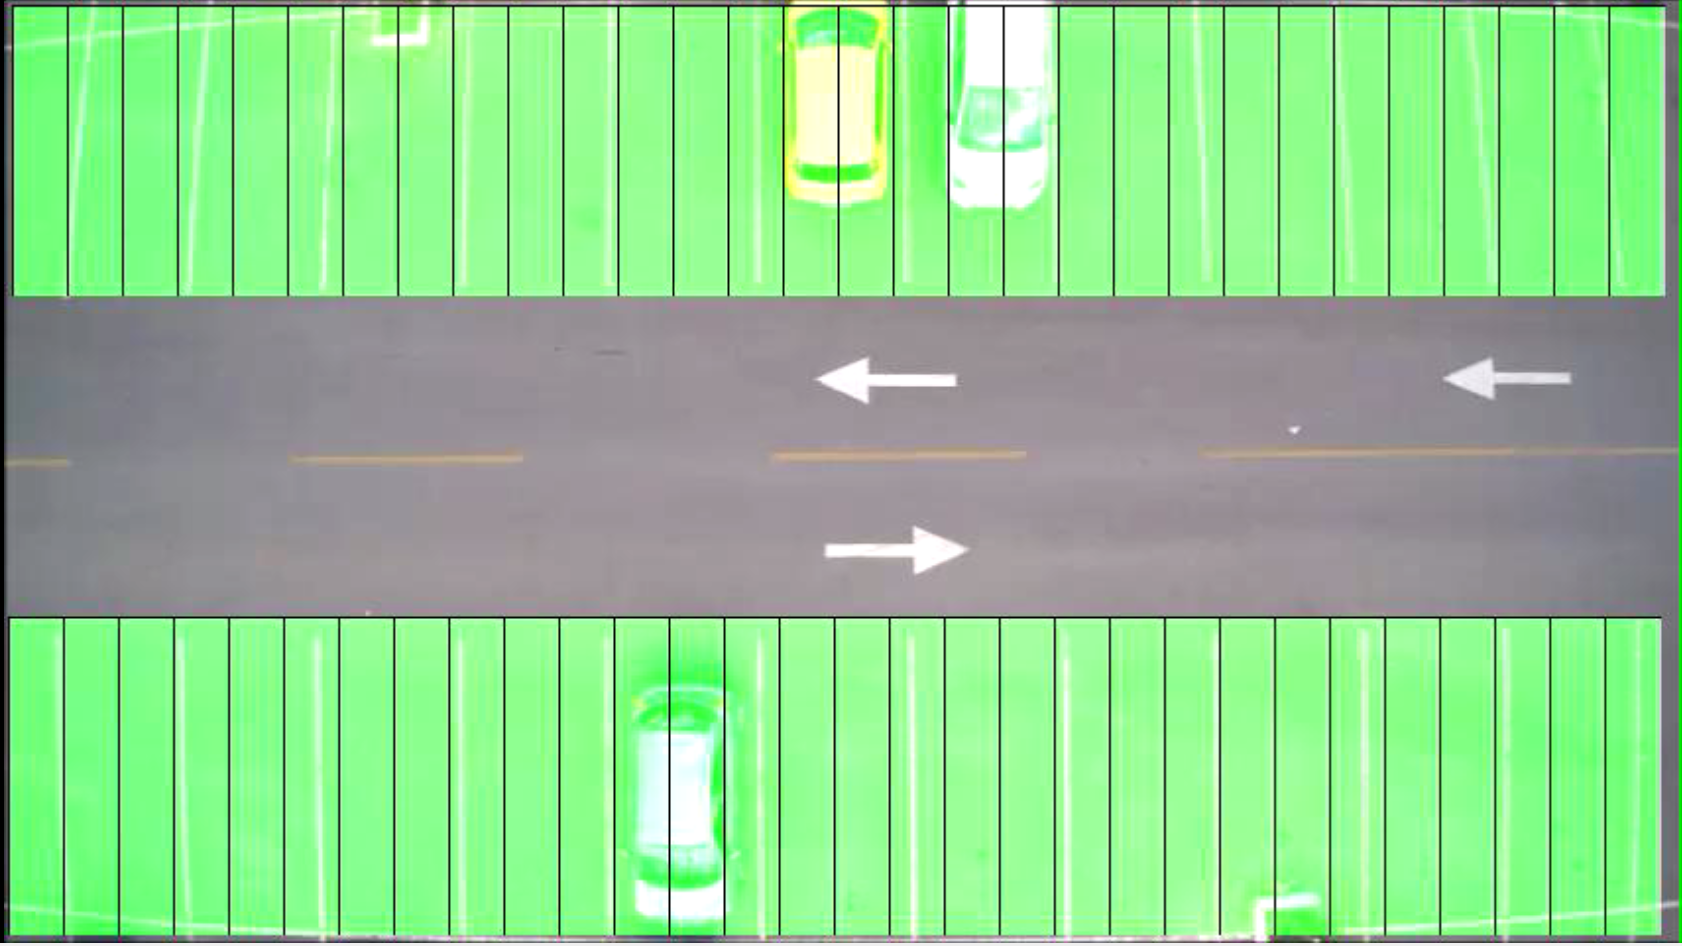
\includegraphics[width=.8\linewidth]{Video5Inicio}
\caption{}
\end{subfigure}\
\begin{subfigure}{.5\textwidth}
\centering
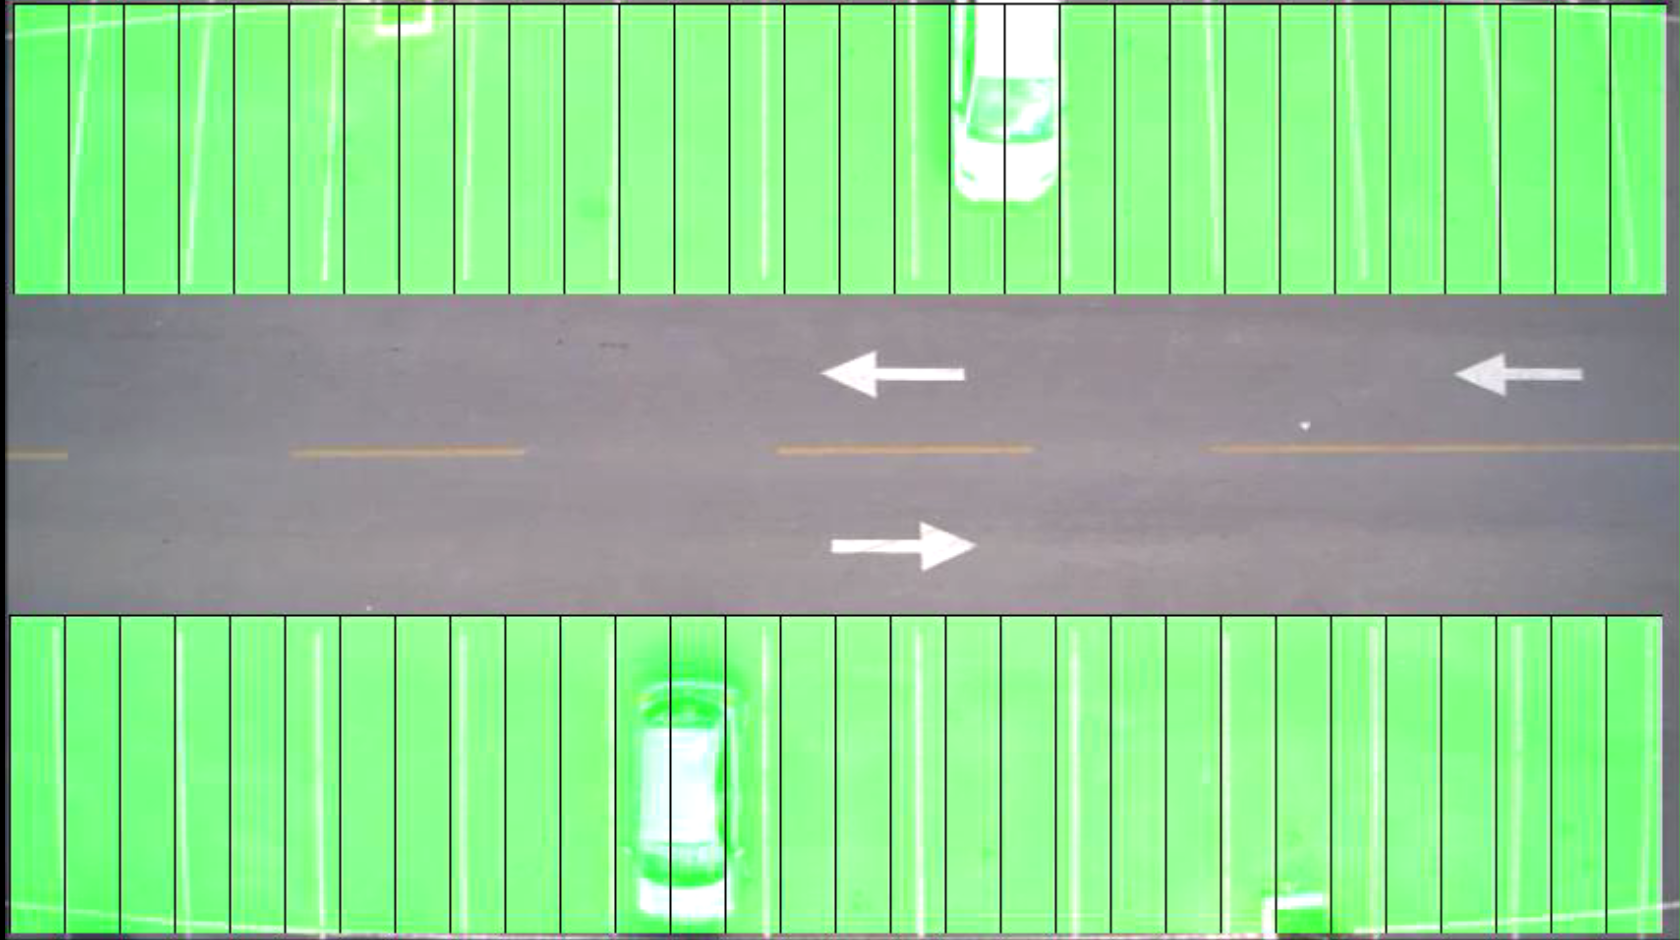
\includegraphics[width=.8\linewidth]{Video5Fim}
\caption{}
\end{subfigure}
\centering
\caption{(a) O momento inicial do vídeo 5; (b) O momento final do vídeo 5.}%
\label{}%
\end{figure}

\begin{center}
\begin{tabular}{|c||c||c|}
\hline
\multicolumn{3}{|c|}{Observador F}  \\ \hline \hline
Tempo(s) & Acontecimento & Vagas Ocupadas\\ \hline
0 & ROI 1: Seções 15,16,18 e 19 ocupadas. & 3 \\
 & ROI 2: Seções 12 e 13 ocupadas. &  \\ \hline
3 & ROI 1: Seções 15 e 16 liberadas. & 2 \\
\hline
\end{tabular}
\end{center}

\begin{center}
\begin{tabular}{|c||c||c|}
\hline
\multicolumn{3}{|c|}{Observador P}  \\ \hline \hline
Tempo(s) & Acontecimento & Vagas Ocupadas\\ \hline
0 & ROI 1: Seções 15,16,18 e 19 ocupadas. & 3 \\
 & ROI 2: Seções 12,13 e 14 ocupadas. &  \\ \hline
4 & ROI 1: Seções 15 e 16 liberadas. & 2 \\
\hline
\end{tabular}
\end{center}

\begin{center}
\begin{tabular}{|c||c||c|}
\hline
\multicolumn{3}{|c|}{Observador M}  \\ \hline \hline
Tempo(s) & Acontecimento & Vagas Ocupadas\\ \hline
0 & ROI 1: Seções 15,16,18 e 19 ocupadas. & 3 \\
 & ROI 2: Seções 12,13 e 14 ocupadas. &  \\ \hline
3 & ROI 1: Seções 15 e 16 liberadas. & 2 \\
\hline
\end{tabular}
\end{center}

\begin{center}
\begin{tabular}{|c||c||c|}
\hline
\multicolumn{3}{|c|}{DVE}  \\ \hline \hline
Tempo(s) & Acontecimento & Vagas Ocupadas\\ \hline
0 & ROI 1: Seções 15,16,18 e 19 ocupadas. & 3 \\
 & ROI 2: Seções 12 e 13 ocupadas. &  \\ \hline
1 & ROI 1: Seção 17 ocupada. & 3 \\ \hline
3 & ROI 1: Seções 15 e 16 liberadas. & 2 \\ \hline
4 & ROI 1: Seção 17 liberada. & 2 \\
\hline
\end{tabular}
\end{center}

\begin{center}
\begin{tabular}{|c||c||c|}
\hline
\multicolumn{3}{|c|}{Acertos - seções}  \\ \hline
Observador & Acertos & Taxa de acertos \\ \hline
F & 597 & 99,50\% \\  \hline
P & 585 & 97,50\% \\ \hline
M & 587 & 97,83\% \\ \hline
Média & 1757 & 97,61\% \\
\hline
\end{tabular}
\end{center}

\begin{center}
\begin{tabular}{|c||c||c|}
\hline
\multicolumn{3}{|c|}{Acertos - vagas}  \\ \hline \hline
Observador & Acertos & Taxa de acertos \\ \hline
F & 10 & 100\% \\  \hline
P & 9 & 90\% \\ \hline
M & 10 & 100\% \\ \hline
Média & 9,66 & 96,66\% \\
\hline
\end{tabular}
\end{center}


Um caso de testes simples, onde os erros ocorreram principalmente por causa da natureza subjetiva do que configura uma seção ocupada. O \textit{DVE} classifica a seção $17$ como ocupada e os observadores não. Por outro lado, dois dos observadores acharam que a seção $14$ da ROI $2$ estava ocupada, descordando do programa. Contudo, essas discordâncias não afetam a quantidade de vagas ocupadas.

\subsection{Vídeo 6}

Neste vídeo o veículo amarelo entra na cena pela parte inferior da tela. O veículo branco desocupa sua vaga e sai da tela pelo lado esquerdo. O vídeo tem $13s$ totalizando $780$ acertos possíveis.

\begin{figure}[!h]
\centering
\begin{subfigure}{.5\textwidth}
\centering
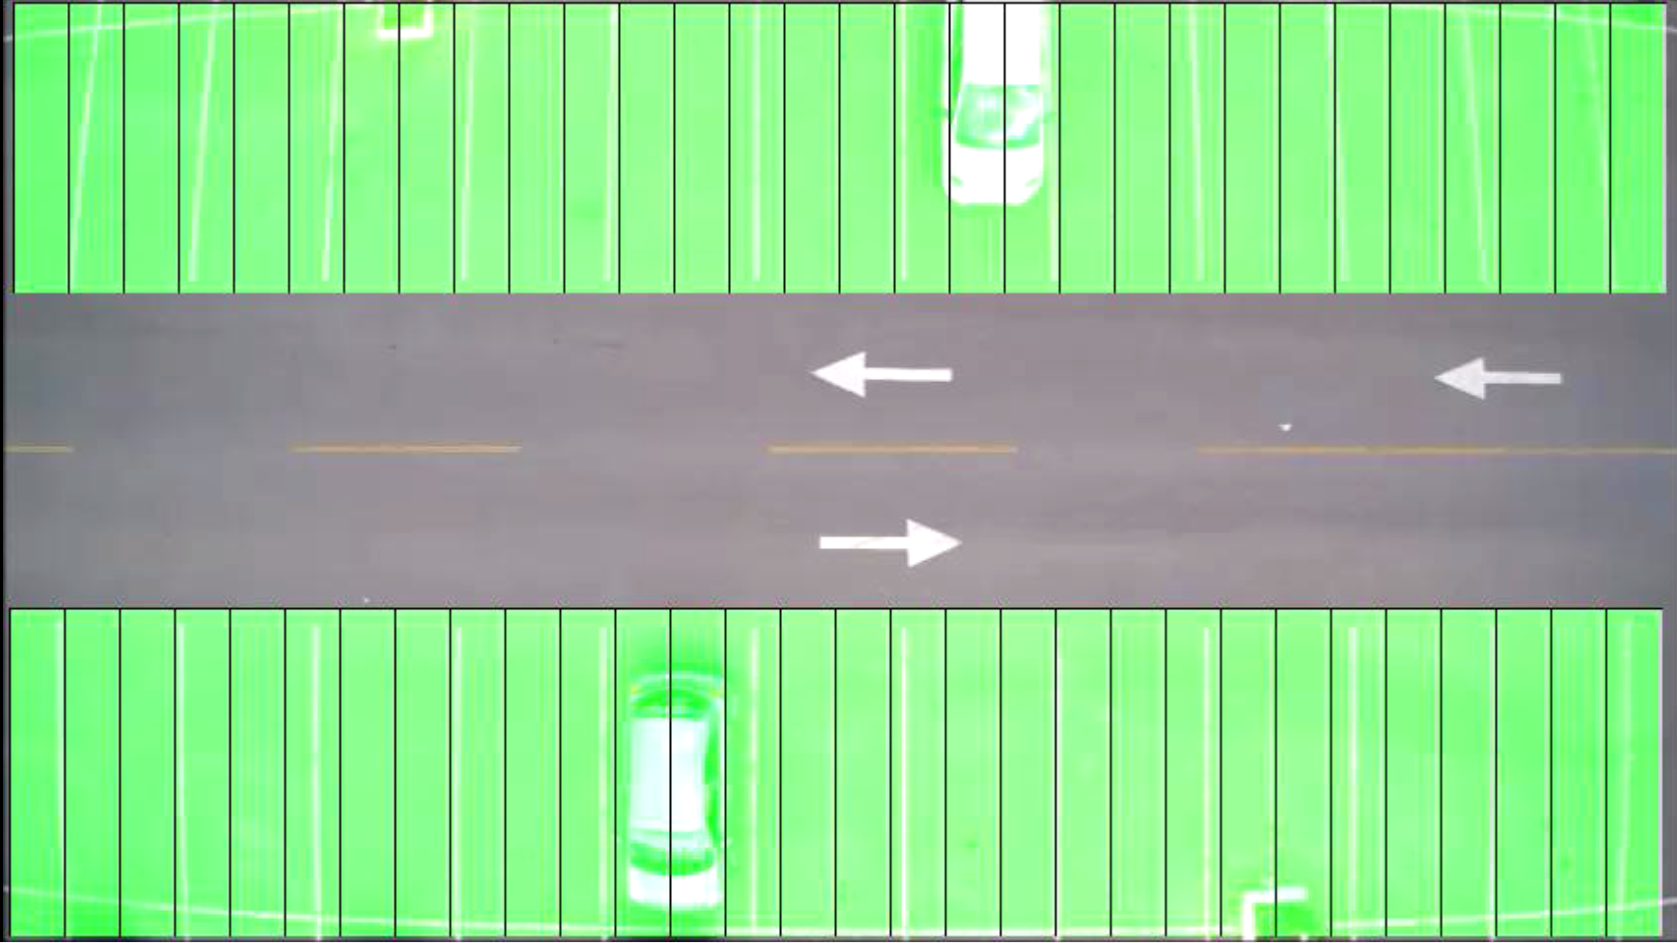
\includegraphics[width=.8\linewidth]{Video6Inicio}
\caption{}
\end{subfigure}\
\begin{subfigure}{.5\textwidth}
\centering
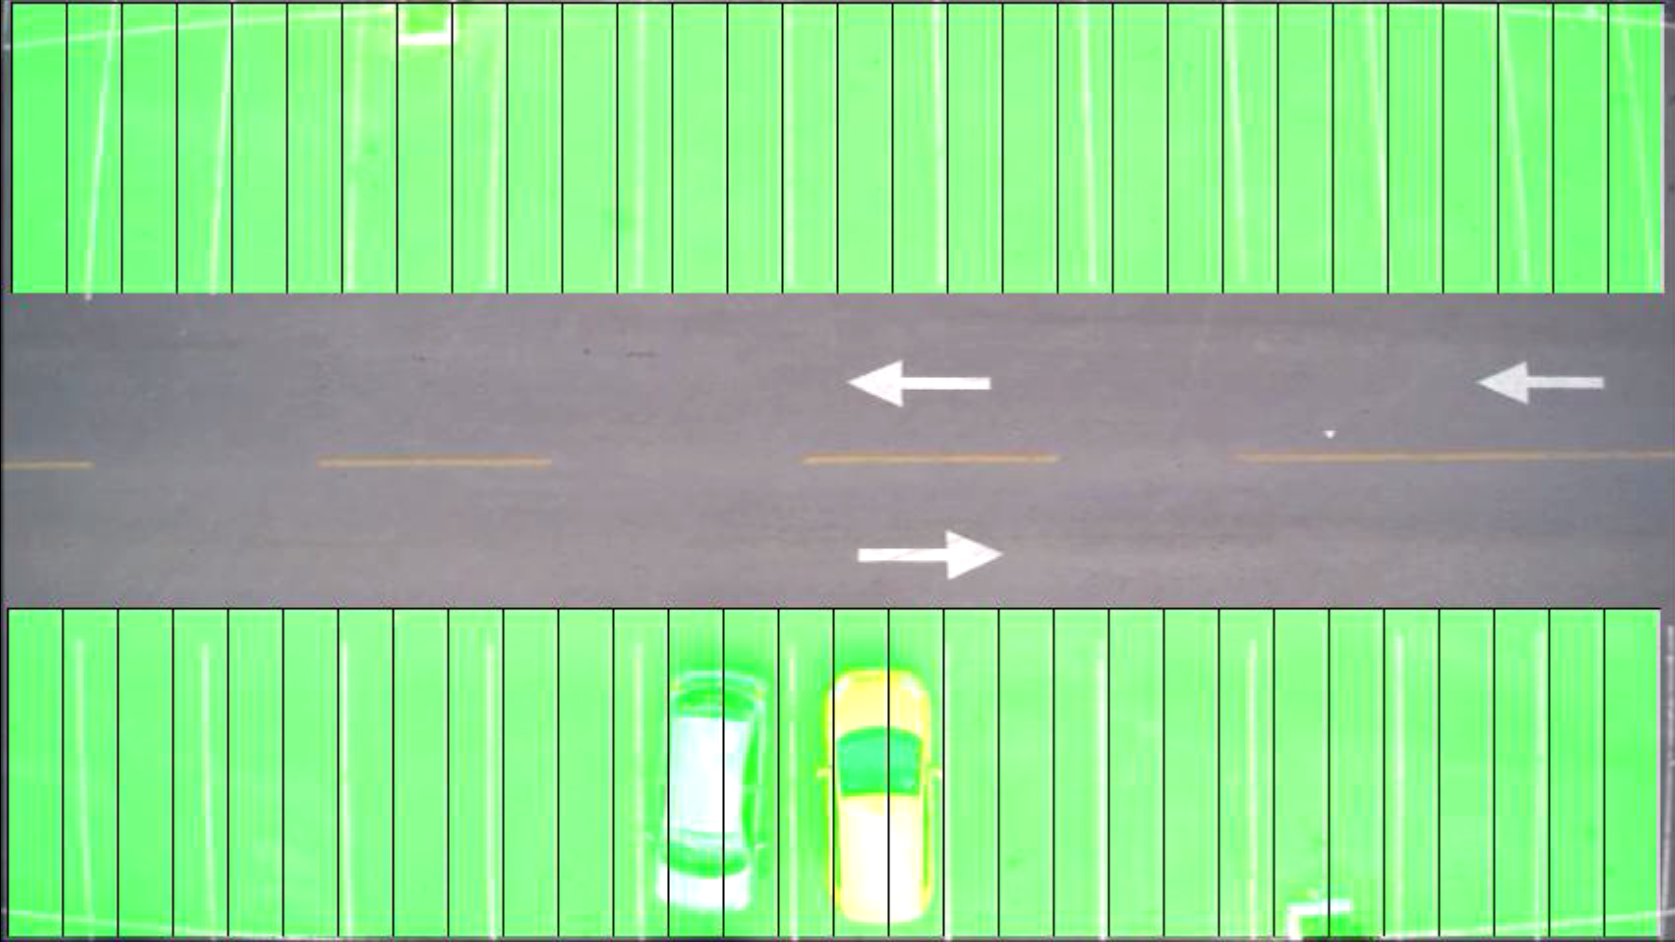
\includegraphics[width=.8\linewidth]{Video6Fim}
\caption{}
\end{subfigure}
\centering
\caption{(a) O momento inicial do vídeo 6; (b) O momento final do vídeo 6.}%
\label{}%
\end{figure}

\begin{center}
\begin{tabular}{|c||c||c|}
\hline
\multicolumn{3}{|c|}{Observador F}  \\ \hline \hline
Tempo(s) & Acontecimento & Vagas Ocupadas \\ \hline
0 & ROI 1: Seções 18 e 19 ocupadas. & 2 \\
 & ROI 2: Seções 12 e 13 ocupadas. &  \\ \hline
5 & ROI 2: Seções 14 e 15 ocupadas. & 3 \\ \hline
8 & ROI 1:Seçoes 18 e 19 liberadas. & 2 \\
\hline
\end{tabular}
\end{center}

\begin{center}
\begin{tabular}{|c||c||c|}
\hline
\multicolumn{3}{|c|}{Observador P}  \\ \hline \hline
Tempo(s) & Acontecimento & Vagas Ocupadas \\ \hline
0 & ROI 1: Seções 18 e 19 ocupadas. & 2 \\
 & ROI 2: Seções 12 e 13 ocupadas. &  \\ \hline
5 & ROI 1: Seções 15,16 e 17 ocupadas. & 3 \\ \hline
9 & ROI 2: Seções 18 e 19 liberadas. & 2 \\
\hline
\end{tabular}
\end{center}

\begin{center}
\begin{tabular}{|c||c||c|}
\hline
\multicolumn{3}{|c|}{Observador M}  \\ \hline \hline
Tempo(s) & Acontecimento & Vagas Ocupadas \\ \hline
0 & ROI 1: Seções 18 e 19 ocupadas. & 2 \\
 & ROI 2: Seções 12 e 13 ocupadas. &  \\ \hline
4 & ROI 1: Seções 15,16 e 17 ocupadas. & 3 \\ \hline
8 & ROI 2: Seções 18,19 liberadas. & 2\\
\hline
\end{tabular}
\end{center}

\begin{center}
\begin{tabular}{|c||c||c|}
\hline
\multicolumn{3}{|c|}{DVE}  \\ \hline \hline
Tempo(s) & Acontecimento & Vagas Ocupadas \\ \hline
0 & ROI 1: Seções 18 e 19 ocupadas. & 2 \\
 & ROI 2: Seções 12 e 13 ocupadas. &  \\ \hline
5 & ROI 2: Seções 15 e 16 ocupadas. & 3 \\ \hline
7 & ROI 2: Seção 17 ocupada. & 3 \\ \hline
11 & ROI 1: Seções 18 e 19 liberadas. & 2 \\
\hline
\end{tabular}
\end{center}

\begin{center}
\begin{tabular}{|c||c||c|}
\hline
\multicolumn{3}{|c|}{Acertos - seções}  \\ \hline
Observador & Acertos & Taxa de acertos \\ \hline
F & 752 & 96,40\% \\  \hline
P & 774 & 99,23\% \\ \hline
M & 767 & 98,33\% \\ \hline
Média & 764,33 & 97,99\% \\
\hline
\end{tabular}
\end{center}


\begin{center}
\begin{tabular}{|c||c||c|}
\hline
\multicolumn{3}{|c|}{Acertos - vagas}  \\ \hline \hline
Observador & Acertos & Taxa de acertos \\ \hline
F & 10 & 76,92\% \\  \hline
P & 11 & 84,61\% \\ \hline
M & 9 & 69,23\% \\ \hline
Média & 10 & 76,92\% \\
\hline
\end{tabular}
\end{center}


Um caso de testes aonde a avaliação do \textit{DVE} se mantém estável e concorda quase plenamente com a avaliação dos humanos. Os atraso da detecção da liberação das seções $18$ e $19$ da ROI $2$ e da desocupação da vaga representada por estas seções se deve ao fato de que o movimento do veículo saindo só é considerado finalizado depois que o veículo sai do campo de visão da câmera, o que ocorre alguns momentos depois que os observadores humanos consideraram que ele saiu da vaga.

\subsection{Vídeo 7}

Neste vídeo um dos carros sai da cena pela esquerda. O vídeo tem $17s$ de duração e portanto $1020$ acertos possíveis.

\begin{figure}[!h]
\centering
\begin{subfigure}{.5\textwidth}
\centering
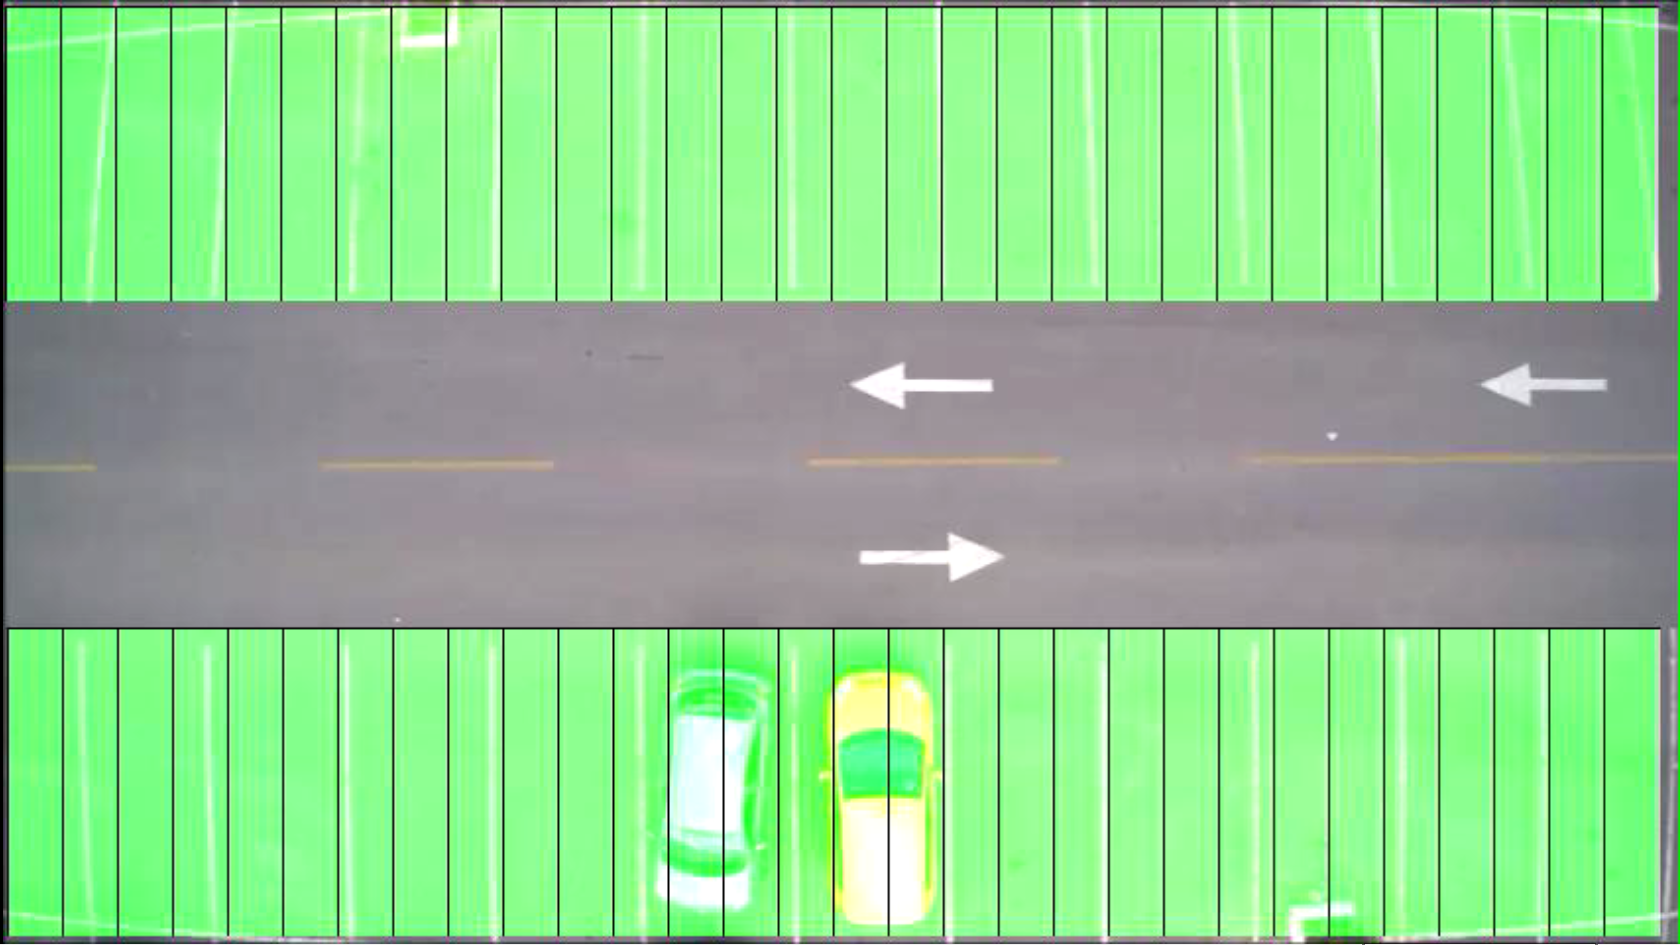
\includegraphics[width=.8\linewidth]{Video7Inicio}
\caption{}
\end{subfigure}\
\begin{subfigure}{.5\textwidth}
\centering
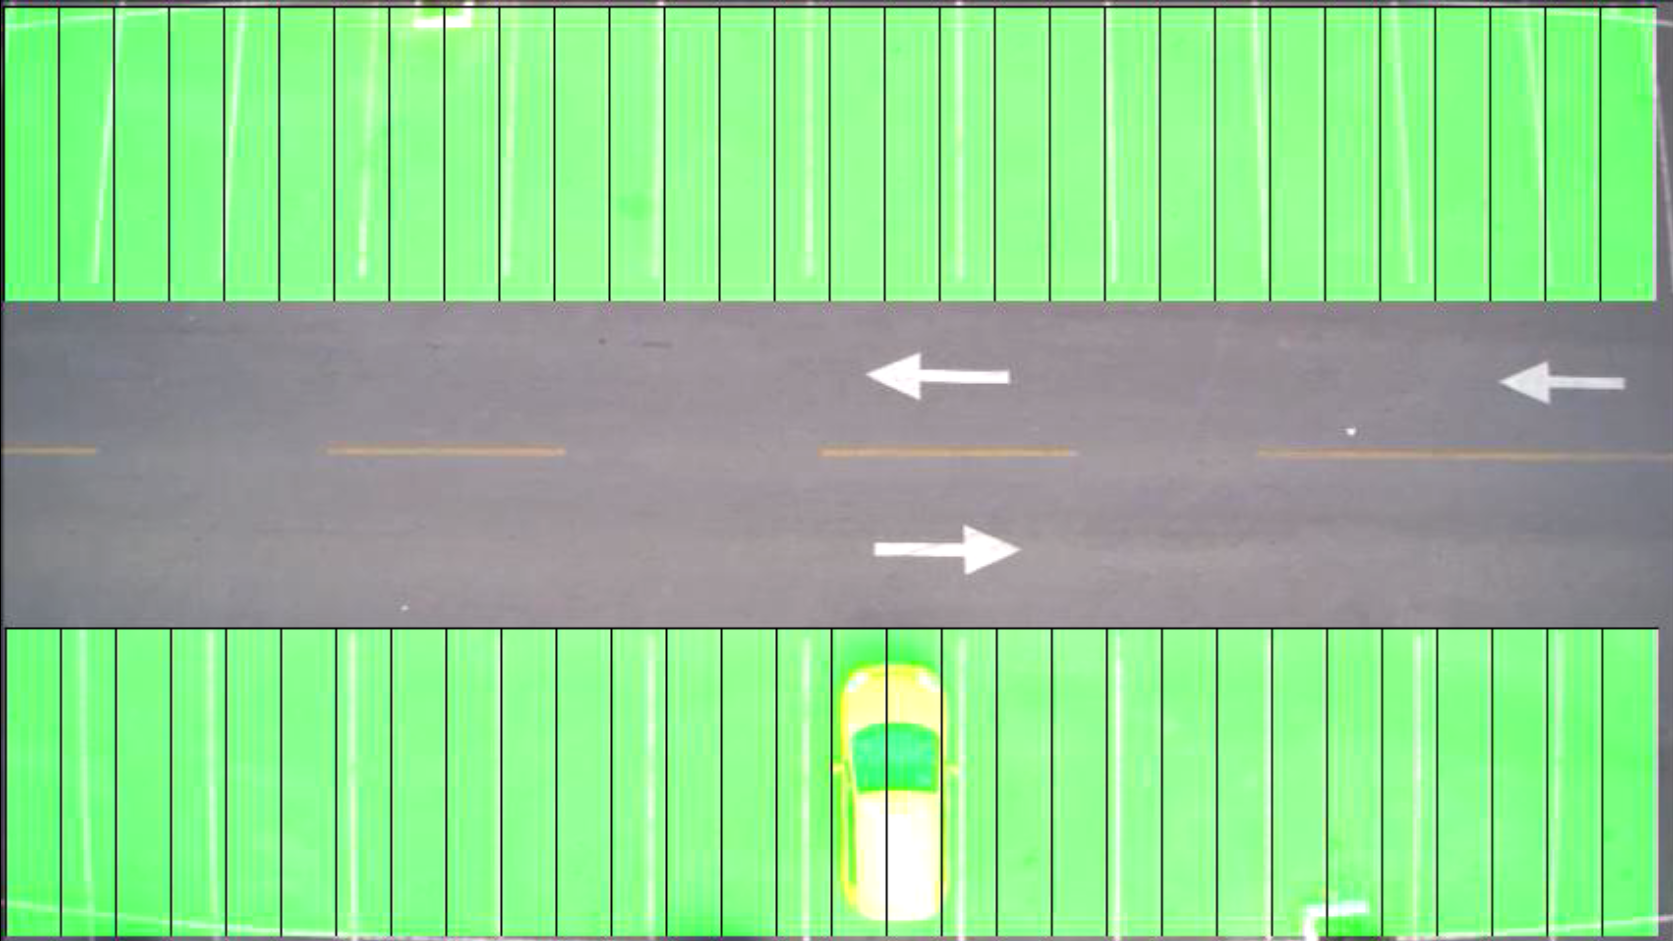
\includegraphics[width=.8\linewidth]{Video7Fim}
\caption{}
\end{subfigure}
\centering
\caption{(a) O momento inicial do vídeo 7; (b) O momento final do vídeo 7.}%
\label{}%
\end{figure}

\begin{center}
\begin{tabular}{|c||c||c|}
\hline
\multicolumn{3}{|c|}{Observador F}  \\ \hline \hline
Tempo(s) & Acontecimento & Vagas Ocupadas \\ \hline
0 & ROI 2: Seções 13,14,16 e 17 ocupadas. & 2 \\ \hline
4 & ROI 2: Seções 13 e 14 liberadas. & 1 \\
\hline
\end{tabular}
\end{center}

\begin{center}
\begin{tabular}{|c||c||c|}
\hline
\multicolumn{3}{|c|}{Observador P}  \\ \hline \hline
Tempo(s) & Acontecimento & Vagas Ocupadas \\ \hline
0 & ROI 2: Seções 12,13,14,16 e 17 ocupadas. & 2 \\ \hline
6 & ROI 2: Seções 12,13,14 liberadas. & 1 \\ 
\hline
\end{tabular}
\end{center}

\begin{center}
\begin{tabular}{|c||c||c|}
\hline
\multicolumn{3}{|c|}{Observador M}  \\ \hline \hline
Tempo(s) & Acontecimento & Vagas Ocupadas \\ \hline
0 & ROI 2: Seções 12,13,14,16 e 17 ocupadas. & 2 \\ \hline
5 & ROI 2: Seções 12,13,14 liberadas. & 1 \\ 
\hline
\end{tabular}
\end{center}

\begin{center}
\begin{tabular}{|c||c||c|}
\hline
\multicolumn{3}{|c|}{DVE}  \\ \hline \hline
Tempo(s) & Acontecimento & Vagas Ocupadas \\ \hline
0 & ROI 2: Seções 13,14,16 e 17 ocupadas. & 2 \\ \hline
1 & ROI 2: Seção 12 ocupada. & 2 \\ \hline
2 & ROI 2: Seção 14 liberada. & 2 \\ \hline
5 & ROI 2: Seções 12 e 13 liberadas. & 1 \\
\hline
\end{tabular}
\end{center}

\begin{center}
\begin{tabular}{|c||c||c|}
\hline
\multicolumn{3}{|c|}{Acertos - seções}  \\ \hline
Observador & Acertos & Taxa de acertos \\ \hline
F & 1013 & 99,31\% \\  \hline
P & 1014 & 99,41\% \\ \hline
M & 1016 & 99,60\% \\ \hline
Média & 1014,33 & 99,44\% \\
\hline
\end{tabular}
\end{center}

\begin{center}
\begin{tabular}{|c||c||c|}
\hline
\multicolumn{3}{|c|}{Acertos - vagas}  \\ \hline \hline
Observador & Acertos & Taxa de acertos \\ \hline
F & 16 & 94,11\% \\  \hline
P & 16 & 94,11\% \\ \hline
M & 17 & 100\% \\ \hline
Média & 16,33 & 96,07\% \\
\hline
\end{tabular}
\end{center}

O programa concordou com os observadores nesse vídeo, exibindo apenas um leve atraso para a classificação correta da seção $12$ e uma liberação levemente precipitada da seção $14$. A ocupação das vagas é determinada de forma quase idêntica a dos observadores.

\subsection{Vídeo 8}

No oitavo e último caso de testes, um carro branco passa pela região central da imagem sem estacionar em nenhuma vaga e depois um carro cinza estaciona na região inferior. O vídeo tem $23s$ de duração e $1380$ acertos possíveis.

\begin{figure}[!h]
\centering
\begin{subfigure}{.5\textwidth}
\centering
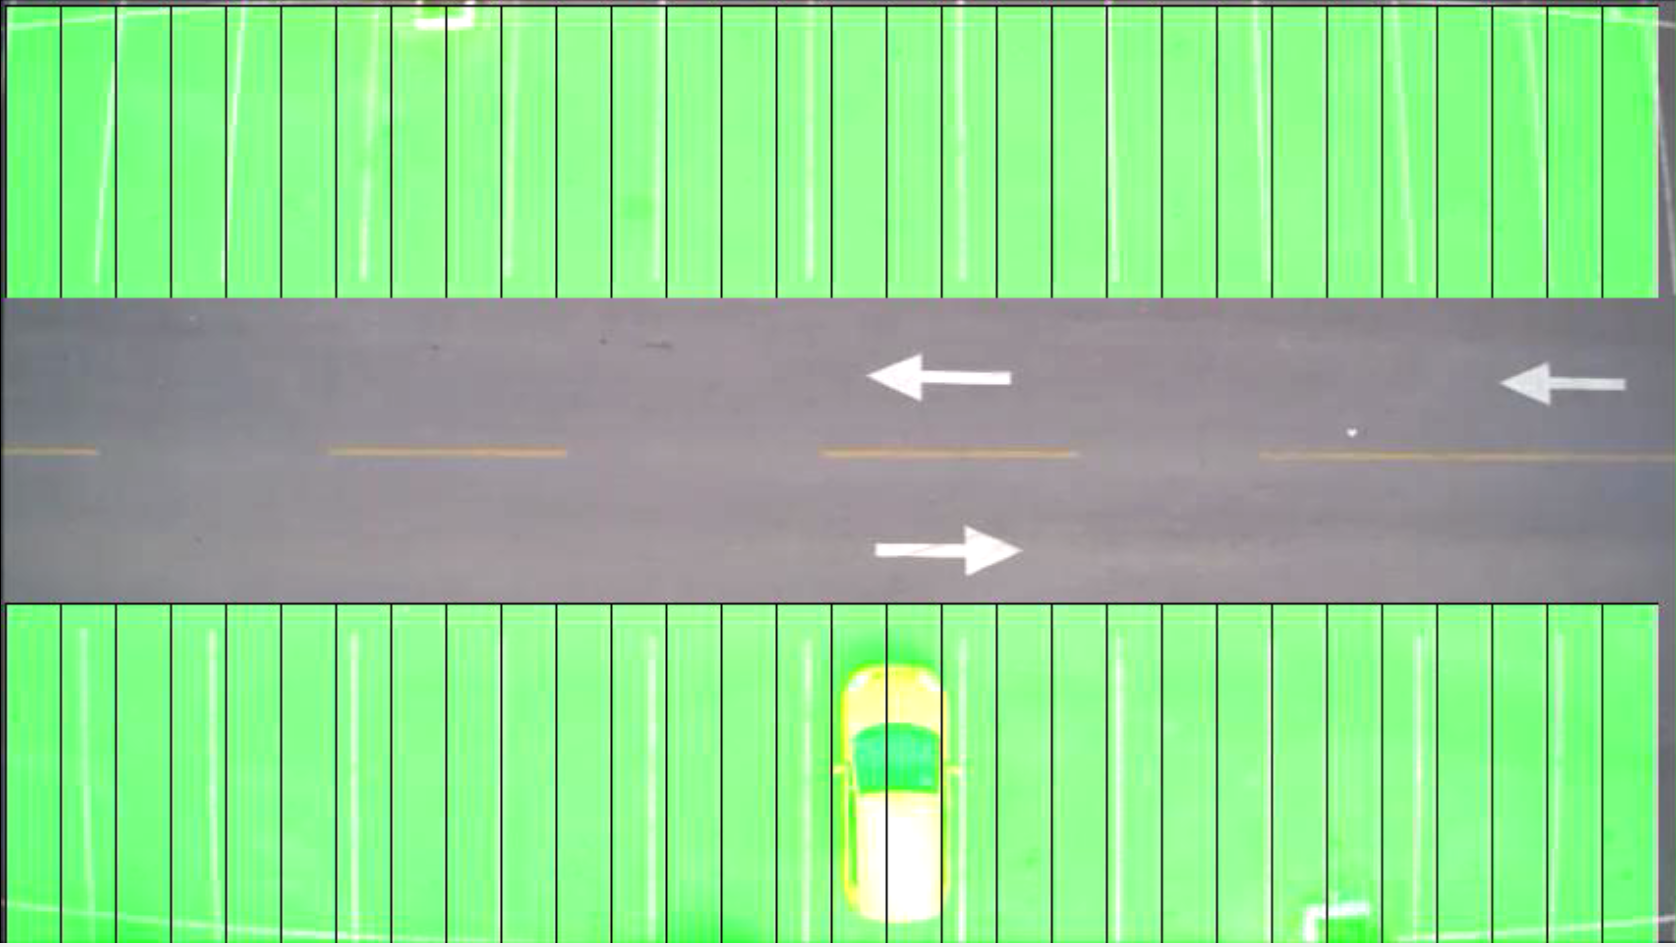
\includegraphics[width=.8\linewidth]{Video8Inicio}
\caption{}
\end{subfigure}\
\begin{subfigure}{.5\textwidth}
\centering
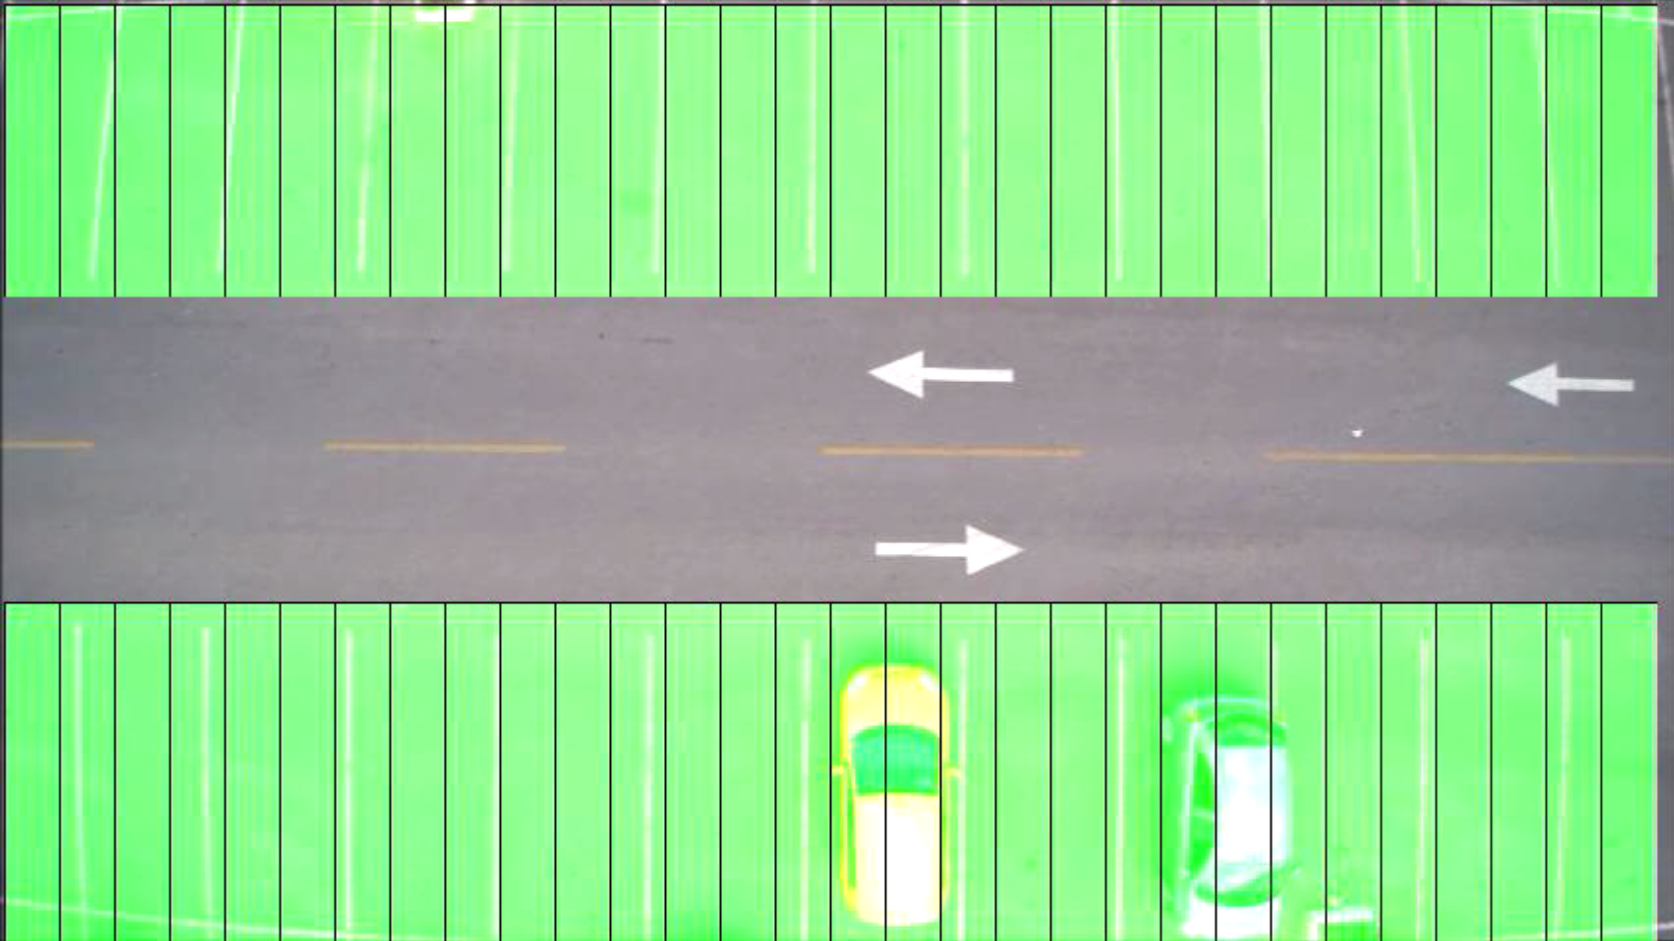
\includegraphics[width=.8\linewidth]{Video8Fim}
\caption{}
\end{subfigure}
\centering
\caption{(a) O momento inicial do vídeo 8; (b) O momento final do vídeo 8.}%
\label{}%
\end{figure}

\begin{center}
\begin{tabular}{|c||c||c|}
\hline
\multicolumn{3}{|c|}{Observador F}  \\ \hline \hline
Tempo(s) & Acontecimento & Vagas Ocupadas\\ \hline
0 & ROI 2: Seções 16 e 17 ocupadas. & 1 \\ \hline
20 & ROI 2: Seções 22 e 23 ocupadas. & 2 \\
\hline
\end{tabular}
\end{center}

\begin{center}
\begin{tabular}{|c||c||c|}
\hline
\multicolumn{3}{|c|}{Observador P}  \\ \hline \hline
Tempo(s) & Acontecimento & Vagas Ocupadas\\ \hline
0 & ROI 2: Seções 16 e 17 ocupadas. & 1 \\ \hline
20 & ROI 2: Seções 22 , 23 e 24 ocupadas. & 2 \\
\hline
\end{tabular}
\end{center}

\begin{center}
\begin{tabular}{|c||c||c|}
\hline
\multicolumn{3}{|c|}{Observador M}  \\ \hline \hline
Tempo(s) & Acontecimento & Vagas Ocupadas\\ \hline
0 & ROI 2: Seções 16 e 17 ocupadas. & 1 \\ \hline
20 & ROI 2: Seções 22,23 e 24 ocupadas. & 2 \\
\hline
\end{tabular}
\end{center}

\begin{center}
\begin{tabular}{|c||c||c|}
\hline
\multicolumn{3}{|c|}{DVE}  \\ \hline \hline
Tempo(s) & Acontecimento & Vagas Ocupadas\\ \hline
0 & ROI 2: Seções 16 e 17 ocupadas. & 1 \\ \hline
20 & ROI 2: Seções 21,22,23 e 24 ocupadas. & 2 \\ \hline
21 & ROI 2: Seção 21 liberada. & 2 \\
\hline
\end{tabular}
\end{center}

\begin{center}
\begin{tabular}{|c||c||c|}
\hline
\multicolumn{3}{|c|}{Acertos - seções}  \\ \hline\hline
Observador & Acertos & Taxa de acertos \\ \hline
F & 1376 & 99,71\% \\  \hline
P & 1379 & 99,92\% \\ \hline
M & 1379 & 99,92\% \\ \hline
Média & 1378 & 99,85\% \\
\hline
\end{tabular}
\end{center}

\begin{center}
\begin{tabular}{|c||c||c|}
\hline
\multicolumn{3}{|c|}{Acertos - vagas}  \\ \hline \hline
Observador & Acertos & Taxa de acertos \\ \hline
F & 23 & 100\% \\  \hline
P & 23 & 100\% \\ \hline
M & 23 & 100\% \\ \hline
Média & 23 & 100\% \\
\hline
\end{tabular}
\end{center}

O programa avalia as seções de forma quase idêntica aos humanos. Aos $20s$, a classificação que ocorre regularmente determina que quatro seções estão sendo ocupadas pelo veículo. Um segundo depois porém, quando o movimento do veículo termina, o erro é corrigido e o programa volta a acertar completamente.











